%% ======================================================================
%% Journal of Computational Physics submission -- cas-sc (CAS Bundle)
%% Skeleton rebuilt from the official CAS template; content migrated
%% from manuscript-0910.tex:
%%   KEPT:      Section 2, Section 3 intro + 3.1 + 3.2
%%   REWRITE:   abstract, highlights, Introduction, Section 3.3 onwards
%% This revision added Sections 3.4--3.6 (time integration, inter-level
%%   transfer & mesh management incl. child-volume check, solution
%%   procedure with Algorithm 1); abstract/roadmap aligned (fixed-topology
%%   accuracy verification added as Section 5); efficiency section annotated with wall-clock
%%   provenance and configuration labels.  New text is marked in red.
%% ======================================================================
% !TeX program = pdflatex
\documentclass[a4paper]{cas-sc}

\usepackage[numbers,sort&compress]{natbib}
\usepackage{xcolor}
\newcommand{\rev}[1]{\textcolor{red}{#1}}

%%% Author macros
\usepackage{subcaption}
\usepackage{epstopdf}
\usepackage{pgfplots}
\usepgfplotslibrary{groupplots}
\pgfplotsset{compat=1.18}
\usepackage{enumitem}
\usepackage[section]{placeins}
% Pseudocode: algorithm2e.sty is not installed in this MiKTeX (package
% database locked); Algorithm 1 is typeset with a zero-dependency ruled
% construction and a manual counter.  To switch back once available:
%   \usepackage[ruled,linesnumbered]{algorithm2e}
\newcounter{algorithm}

% Figure placement parameters
\renewcommand{\topfraction}{.9}
\renewcommand{\bottomfraction}{.8}
\renewcommand{\textfraction}{.05}
\renewcommand{\floatpagefraction}{.6}
\setcounter{topnumber}{9}
\setcounter{bottomnumber}{9}
\setcounter{totalnumber}{20}
\setlength{\floatsep}{8pt plus 2pt minus 2pt}
\setlength{\textfloatsep}{8pt plus 2pt minus 2pt}
\setlength{\intextsep}{8pt plus 2pt minus 2pt}

\begin{document}
\let\WriteBookmarks\relax

% Short title
\shorttitle{A Conservative Flux Closure for Cell-Centered Lagrangian AMR}

% Short author
\shortauthors{C.~Xu}

% Main title of the paper
\title[mode = title]{Conservative hanging-node flux closure and dimensionless refinement criterion
for cell-centered Lagrangian AMR}

\author[1]{Chunyuan Xu}[orcid=0000-0002-9089-2852]

% Corresponding author indication
\cormark[1]

% Email id of the first author
\ead{xcyuan@mail.ustc.edu.cn}

% Address/affiliation
\affiliation[1]{organization={Institute of Applied Physics and Computational Mathematics},
            city={Beijing},
            country={China}}

% Corresponding author text
\cortext[1]{Corresponding author}

\begin{abstract}
Coupling adaptive mesh refinement (AMR) with Lagrangian hydrodynamics is difficult because the mesh moves with the flow: a coarse--fine interface is a moving internal boundary that participates in the flux exchange, so adaptation must preserve both the conservation laws and the geometric consistency of the embedded hierarchy. In cell-centered Lagrangian schemes, nodes carry no independent physical variables, which allows hanging points to be treated as purely geometric points slaved to their supporting coarse edges. Building on this observation, we construct a flux closure for $2\!:\!1$ non-conforming quadtree meshes in which hanging points carry no degree of freedom: the flux over each boundary segment ending at a hanging point is closed entirely by the half-Riemann relations of the adjacent independent nodes. The closure preserves discrete total energy and momentum conservation and the geometric conservation law of the coarse cells and of each aggregated refined patch. Because the simple quadtree topology --- straight coarse edges and permanently aligned children and parents --- is preserved, conservative refinement and coarsening require no geometric repair. For the adaptation itself, two families of dimensionless sensors---thermodynamic, from the density and pressure jumps, and kinematic, from the velocity divergence---are combined by an OR rule behind a single threshold pair. The closure is verified to first order on fixed-topology non-conforming meshes (Taylor--Green vortex, observed order $0.83\to0.95$), and on three classical shock problems the adaptive calculations match the captured-shock width of the uniformly refined reference at their finest level---within $10\%$ on Sedov and Sod and within $22\%$ on Noh---while using $0.4$--$8\%$ of its cell-steps, with total energy conserved to machine precision on every run.
\end{abstract}

%% Research highlights (Elsevier: 3-5 bullets, max 85 characters each)
\begin{highlights}
\item Hanging nodes on non-conforming quadtree meshes need no independent degree of freedom.
\item Flux closure preserves discrete momentum and energy with no geometric repair.
\item One dimensionless threshold pair adapts ahead of shocks without problem-specific tuning.
\item Uniform-grid front resolution at 0.4--8\% of its cell-steps, energy exact to round-off.
\end{highlights}

% Keywords
\begin{keywords}
Lagrangian hydrodynamics \sep Adaptive mesh refinement \sep Cell-centered scheme \sep Hanging nodes \sep Flux closure \sep Conservative method
\end{keywords}

\maketitle

%% ======================================================================
%  SECTION 1: INTRODUCTION
%% ======================================================================
\section{Introduction}
\label{sec:introduction}

Shock-dominated compressible flows, as arise in high-energy-density physics, inertial confinement fusion, and astrophysics, concentrate their essential dynamics into thin, strongly localized fronts whose thickness is far below any affordable mesh size. Because uniformly fine grids are prohibitively expensive for such flows, adaptive mesh refinement (AMR) has been central to computational gas dynamics since its inception: Berger and Oliger~\cite{berger1984adaptive} and Berger and Colella~\cite{berger1989local} introduced block-structured hierarchies driven by local error estimates and equipped with interface flux corrections, which were extended to three dimensions~\cite{bell1994three} and to Cartesian grids over irregular geometries~\cite{pember1995adaptive}; tree-based formulations~\cite{khokhlov1998fully,burstedde2011p4est} refine individual cells and today underpin large-scale adaptive frameworks.

Lagrangian and arbitrary Lagrangian--Eulerian (ALE) methods~\cite{hirt1974arbitrary,benson1992computational} approach the same resolution problem from the opposite direction: the mesh moves synchronously with the flow, following shocks and material interfaces and gathering cells into the compressed regions behind them~\cite{vonneumann1950method,wilkins1964calculation,caramana1998construction}. This adaptivity through motion, however, redistributes a fixed number of cells: it changes where the resolution resides, not how much of it exists, and the accuracy of a calculation remains bounded by its initial mesh. AMR, by contrast, injects resolution where and when it is needed. Coupling the two is therefore attractive, and Lagrangian--AMR calculations have been shown to recover uniformly refined accuracy at a fraction of its cost~\cite{anderson2004arbitrary,morrell2007cell,waltz2018coupled}; yet published couplings remain scarce~\cite{anderson2004arbitrary,morrell2007cell,koniges2006modeling,wang2010modeling,baiges2017adaptive,waltz2018coupled,colaitis2026cell}.

The scarcity has a structural reason. In Eulerian AMR the mesh is stationary, and a coarse--fine interface is a data interface, handled through ghost-cell interpolation and flux corrections at grid interfaces~\cite{berger1989local,berger1987conservation}. In a Lagrangian calculation, by contrast, the mesh moves synchronously with the flow, so a coarse--fine interface is a moving internal boundary that directly participates in the exchange of momentum and energy; refinement and coarsening, moreover, modify the mesh topology locally while the mesh is being advected. The central difficulty of Lagrangian AMR is thus to preserve, throughout adaptation, the physical conservation laws and the geometric consistency of the embedded hierarchy at the same time --- the latter expressed by the geometric conservation law (GCL)~\cite{thomas1979geometric,guillard2000significance,farhat2001discrete} and by the child--parent alignment on which volume conservation at coarsening and the invertibility of inter-level transfer operators rest~\cite{anderson2004arbitrary,waltz2018coupled}.

Existing coarse--fine treatments can be classified by the status they assign to hanging points. Anderson et al.~\cite{anderson2004arbitrary} employ structured patch AMR: each level advances independently and couples to its neighbors only through interpolated boundary conditions, which makes the hierarchy natural to operate but leaves discrete conservation across level interfaces unenforced --- a limitation the authors themselves list as future work. Morrell et al.~\cite{morrell2007cell} solve on a single composite mesh; because their staggered discretization assigns mass and forces to nodes, hanging nodes have no independent status, and the mass and force they gather must be redistributed to the adjacent master nodes --- a treatment whose velocity interpolation does not conserve momentum. Waltz and Bakosi~\cite{waltz2018coupled} remove hanging points altogether by iteratively refining neighbors until the mesh is conformal, at the price of a diffused refinement region and constrained motion of refinement points. Most recently, Cola{\"i}tis et al.~\cite{colaitis2026cell} couple a conservative cell-centered scheme with an octree forest and let hanging nodes move freely exactly like any other node: the baseline scheme~\cite{georges2016three} applies without any modification and its conservation properties carry over verbatim, at the cost of a heavy topology management --- cells of up to twenty-four faces --- together with geometric repairs prior to refinement.

In cell-centered Lagrangian schemes~\cite{maire2007SIAM,maire2009high}, all conserved quantities reside in the cells and nodes carry no independent physical variables; they serve only to close the boundary fluxes. A hanging point can therefore be treated as a purely geometric, dependent point without discarding any physics --- but conservation and geometric consistency do not follow from this observation alone and must be built into the interface closure. In this work we construct such a closure on $2\!:\!1$ balanced quadtree meshes: hanging points are slaved to their supporting coarse edges and carry no independent degree of freedom, and the flux over each boundary segment ending at a hanging point is closed entirely by the half-Riemann relations of the adjacent independent nodes. With this closure, discrete conservation of total energy and momentum holds on meshes containing level interfaces, together with the GCL of the coarse cells and of each aggregated refined patch; the GCL of an individual fine cell is deliberately not enforced, since no degree of freedom is attached to a hanging point. The quadtree topology --- straight coarse edges and permanently aligned children and parents --- is preserved, so that conservative refinement and coarsening require no geometric repair.

Adaptation criteria inherit the same framework mismatch. Criteria designed for the Eulerian setting, whether based on local error estimates~\cite{berger1984adaptive,lohner1987adaptive} or on normalized jumps, do not transpose directly: synchronous mesh motion already compresses discontinuities onto a few cells, so absolute-difference criteria would keep refining fronts that are already resolved~\cite{colaitis2026cell}. Existing Lagrangian AMR codes accordingly employ normalized second differences~\cite{anderson2004arbitrary}, directional density differences~\cite{morrell2007cell}, normalized gradients~\cite{waltz2018coupled}, or composite multi-source metrics~\cite{colaitis2026cell}. We instead draw on all three fields: weighted, normalized pressure and density jumps form a thermodynamic sensor, while the velocity divergence---the classical shock operator of Lagrangian hydrodynamics, equal on a moving mesh to the relative rate of volume change---forms a kinematic sensor; a cell is flagged when either sensor responds. Because the mesh motion supplies sharp raw signals, one common dimensionless measure then separates discontinuities already resolved by the motion from genuinely under-resolved regions ahead of the shock, so that refinement is automatically placed ahead of incoming fronts.

The main contributions of this work are: (i)~a flux closure for non-conforming quadtree interfaces in which hanging points carry no independent degree of freedom and all interface fluxes are closed by the adjacent independent nodes, with discrete total-energy and momentum conservation and the GCL of the coarse cells and of each aggregated refined patch holding on adapted meshes; (ii)~the preservation of the simple quadtree topology across refinement and coarsening --- straight coarse edges and permanent child--parent alignment --- which renders conservative inter-level transfers free of geometric repair; and (iii)~a dimensionless dual-channel refinement indicator---thermodynamic (weighted pressure and density) and kinematic (velocity divergence) sensors aggregated by an OR rule---that concentrates refinement automatically ahead of shock fronts. The two layers are logically independent---conservation is a property of the closure, robustness a property of the solver---and Section~5 isolates the closure from remeshing altogether by freezing the mesh topology after a single refinement. The remainder of the paper is organized as follows. Section~2 reviews the governing equations and the baseline cell-centered Lagrangian scheme. Section~3 develops the nodal flux closure at non-conforming interfaces, its explicit time integration, and the conservative inter-level transfers. Section~4 presents the refinement indicator, Section~5 verifies the accuracy of the scheme on fixed-topology non-conforming meshes, Section~6 assesses the adaptive scheme numerically, and Section~7 concludes.

\section{Governing Equations and Baseline Cell-Centered Lagrangian Scheme}
\label{sec:baseline}

\subsection{Governing equations}
\label{sec:governing}

The two-dimensional Lagrangian equations of gas dynamics for an inviscid, compressible fluid describe the conservation of volume, mass, momentum, and energy in a moving frame. For a control volume $\Omega(t)$ bounded by its closed boundary $\partial\Omega(t)$ with unit outward normal $\boldsymbol{N}$, the integral conservation laws are:

\begin{subequations}
	\begin{align}
		\frac{d}{dt} \int_{\Omega} d\Omega - \int_{\partial\Omega} \boldsymbol{U} \cdot \boldsymbol{N} \, dL &= 0, \label{eq:gov_vol}\\
		\frac{d}{dt} \int_{\Omega} \rho \, d\Omega &= 0, \label{eq:gov_mass}\\
		\frac{d}{dt} \int_{\Omega} \rho \boldsymbol{U} \, d\Omega + \int_{\partial\Omega} P \boldsymbol{N} \, dL &= 0, \label{eq:gov_mom}\\
		\frac{d}{dt} \int_{\Omega} \rho E \, d\Omega + \int_{\partial\Omega} P \boldsymbol{U} \cdot \boldsymbol{N} \, dL &= 0. \label{eq:gov_ene}
	\end{align}
	\label{eq:gov_all}
\end{subequations}
where $t$ represents time, $\rho$ is the fluid density, $P$ is the pressure, $\boldsymbol{U}$ is the velocity vector, $E$ is the specific total energy, and $dL$ is the length element along the boundary. Equation~\eqref{eq:gov_vol} represents the Geometric Conservation Law (GCL). The system is closed by a thermodynamic equation of state (EOS): $P = P(\rho, e)$, where the specific internal energy is $e = E - \frac{1}{2}|\boldsymbol{U}|^2$. For an ideal gas, the pressure is given by
\begin{equation}
		P = (\gamma-1)\rho e,
		\label{eq:eos_ideal}
	\end{equation}
	where $\gamma$ denotes the adiabatic index.

\subsection{The cell-centered Lagrangian scheme on conforming quadrilateral meshes}
\label{sec:cch}

Our flux closure condition builds on the cell-centered Lagrangian hydrodynamics (CCH) scheme of Maire et al.~\cite{maire2007SIAM}. This section reviews the baseline discretization on conforming quadrilateral meshes, establishing the notation and the conservation framework into which the flux closure condition will be embedded.

\subsubsection{Notation and assumptions}
\label{sec:notations}

The two-dimensional spatial domain is discretized into quadrilateral cells. Each cell, denoted by $\Omega_c$, is assigned a unique index $c$, and each vertex is assigned a unique index $p$. As shown in Fig.~\ref{fig:basic_notation}, for a given cell $\Omega_c$ and a node $p \in \mathcal{P}(c)$ (where $\mathcal{P}(c)$ is the set of vertices of cell $c$), the two neighboring vertices along the cell boundary are denoted by $p^+$ and $p^-$ (in the counterclockwise and clockwise directions, respectively).

\begin{itemize}
	\item \textbf{Fluid Variables and Lagrangian Mass:} The thermodynamic and dynamic state of cell $c$ is defined by the cell-centered density $\rho_c$, pressure $P_c$, specific total energy $E_c$, and velocity vector $\boldsymbol{U}_c$. The cell mass $m_c = \rho_c(t) V_c(t)$ is invariant in time, where $V_c(t)$ is the cell volume. For any vertex $p \in \mathcal{P}(c)$, its kinematic state is specified by position $\boldsymbol{X}_p(t)$ and velocity $\boldsymbol{U}_p$.
	
	\item \textbf{Half-Edge Notation:} Each cell boundary edge at node $p$ is split into half-segments. Let $L_{pp^{\pm}}$ and $\boldsymbol{N}_{pp^{\pm}}^c$ be the total lengths and unit outward normals of the adjacent edges with respect to cell $c$. The subcell half-edge lengths and unit outward normals are defined as:
	\begin{equation}
		L_{\overline{p}}^c = \frac{1}{2} L_{pp^+}, \quad \boldsymbol{N}_{\overline{p}}^c = \boldsymbol{N}_{pp^+}^c, \qquad
		L_{\underline{p}}^c = \frac{1}{2} L_{pp^-}, \quad \boldsymbol{N}_{\underline{p}}^c = \boldsymbol{N}_{pp^-}^c.
		\label{eq:halfedge_def}
	\end{equation}
	The subcell half-edge pressures $\Pi_{\overline{p}}^c$ and $\Pi_{\underline{p}}^c$ act as auxiliary thermodynamic variables at the node, which are used to construct the numerical fluxes.
\end{itemize}

Under these definitions, the rate of change of the cell volume $V_c$ is directly linked to the nodal velocities $\boldsymbol{U}_p$~\cite{maire2009high}, enabling a discretization framework that satisfies the GCL.

\begin{figure}[pos=htbp]
	\centering
	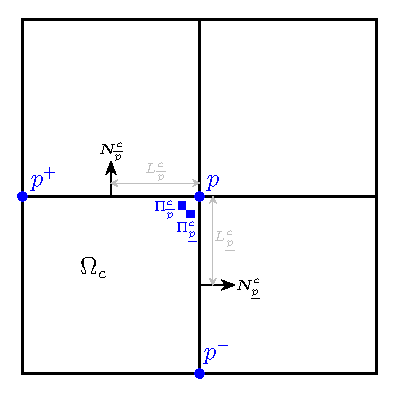
\includegraphics[width=0.45\textwidth]{figure1.pdf}
	\caption{Schematic of the notation for a generic quadrilateral cell $\Omega_c$, showing the subcell parameters $(L_{\overline{p}}^c, \boldsymbol{N}_{\overline{p}}^c, \Pi_{\overline{p}}^c)$ and $(L_{\underline{p}}^c, \boldsymbol{N}_{\underline{p}}^c, \Pi_{\underline{p}}^c)$ associated with node $p$ and its neighbors $p^+$ and $p^-$.}
	\label{fig:basic_notation}
\end{figure}

\subsubsection{Conservation-based nodal solver}

Following Maire et al.~\cite{maire2007SIAM}, a multidimensional acoustic Riemann solver is formulated at each node. For a generic cell $\Omega_c$ sharing node $p$, the subcell half-edge pressures are linearized using a one-dimensional acoustic approximation:
\begin{equation}
	\begin{aligned}
		P_c-\Pi_{\overline{p}}^c &= Z_c (\boldsymbol{U}_p - \boldsymbol{U}_c) \cdot \boldsymbol{N}_{\overline{p}}^c,\\
		P_c-\Pi_{\underline{p}}^c &= Z_c (\boldsymbol{U}_p - \boldsymbol{U}_c) \cdot \boldsymbol{N}_{\underline{p}}^c,
	\end{aligned}
	\label{eq:acoustic}
\end{equation}
where $Z_c = \rho_c a_c$ is the local acoustic impedance, with $a_c$ being the sound speed. The relation is written in pressure-difference form, $P_c-\Pi_s^c=Z_c(\boldsymbol{U}_p-\boldsymbol{U}_c)\cdot\boldsymbol{N}_s^c$, for either half-edge $s$. To ensure momentum conservation of the cell-centered scheme, the subcell forces at node $p$ must sum to zero (force balance at the node):
\begin{equation}
	\sum_{c \in \mathcal{C}(p)} \left( \Pi_{\overline{p}}^c L_{\overline{p}}^c \boldsymbol{N}_{\overline{p}}^c + \Pi_{\underline{p}}^c L_{\underline{p}}^c \boldsymbol{N}_{\underline{p}}^c \right) = \boldsymbol{0},
	\label{eq:momentum_Pi}
\end{equation}
where $\mathcal{C}(p)$ is the set of cells connected to vertex $p$. Substituting Eq.~\eqref{eq:acoustic} into Eq.~\eqref{eq:momentum_Pi} yields the explicit nodal velocity:
\begin{equation}
\boldsymbol{U}_p = \mathsf{M}_p^{-1} \sum_{c \in \mathcal{C}(p)} \left( \mathsf{M}_p^c \boldsymbol{U}_c + P_c L_{p}^c \boldsymbol{N}_{p}^c \right),
	\label{eq:nodalsolver}
\end{equation}
where the corner normal vector $L_p^c \boldsymbol{N}_p^c$, the subcell matrix $\mathsf{M}_p^c$, and the nodal matrix $\mathsf{M}_p$ are defined as:
\begin{equation}
	L_{p}^c \boldsymbol{N}_{p}^c = L_{\overline{p}}^c \boldsymbol{N}_{\overline{p}}^c + L_{\underline{p}}^c \boldsymbol{N}_{\underline{p}}^c,\quad
	\mathsf{M}_p = \sum_{c \in \mathcal{C}(p)} \mathsf{M}_p^c,\quad
	\mathsf{M}_p^c = Z_c \left( L_{\overline{p}}^c \boldsymbol{N}_{\overline{p}}^c \otimes \boldsymbol{N}_{\overline{p}}^c + L_{\underline{p}}^c \boldsymbol{N}_{\underline{p}}^c \otimes \boldsymbol{N}_{\underline{p}}^c \right),
	\label{eq:matrixP}
\end{equation}
with $\otimes$ denoting the tensor product. For any vector $\boldsymbol v$, the quadratic form of $\mathsf M_p^c$ is $Z_c\bigl(L_{\overline p}^c(\boldsymbol v\cdot\boldsymbol N_{\overline p}^c)^2+L_{\underline p}^c(\boldsymbol v\cdot\boldsymbol N_{\underline p}^c)^2\bigr)$, which is non-negative and vanishes only when the two portions meeting at $p$ are collinear; the nodal matrix $\mathsf M_p$ is therefore positive definite and the nodal velocity~\eqref{eq:nodalsolver} is uniquely determined whenever the cell geometry is non-degenerate. Substituting $\boldsymbol{U}_p$ back into Eq.~\eqref{eq:acoustic} closes the nodal solver.

\par\medskip\noindent\textbf{Remark (numerical dissipation).}
The dissipation that captures shocks in this first-order scheme is that of the
Godunov-type acoustic solver itself: the half-Riemann relations~\eqref{eq:acoustic}
already carry the impedance $Z_c=\rho_ca_c$, and no separate artificial-viscosity
term is added. A single scalar control is retained on top of it: the acoustic
impedance may be scaled, $Z_c\leftarrow\kappa_d\,Z_c$, to strengthen the dissipation
of the nodal solve where the sustained convergence of a calculation threatens the
mesh. All calculations use $\kappa_d=1$ except the Noh problem, where every
run---uniform and adaptive alike---uses $\kappa_d=1.5$, so chosen as to carry the
deeply refined uniform grids through the strong central compression; the value is
fixed once per problem and never tuned per level or hierarchy.

\subsection{Spatial discretization on conforming meshes}

The semi-discrete finite volume equations are obtained by integrating the conservation laws over the moving cell $\Omega_c(t)$. For cell $c$, the subcell force exerted at node $p$ is:
\begin{equation}
\boldsymbol{F}_{pc} = \Pi_{\overline{p}}^c L_{\overline{p}}^c \boldsymbol{N}_{\overline{p}}^c + \Pi_{\underline{p}}^c L_{\underline{p}}^c \boldsymbol{N}_{\underline{p}}^c.
	\label{eq:Fcp}
\end{equation}
Since the cell mass $m_c$ is constant, the semi-discrete conservation equations for cell $c$ read:
\begin{subequations}
	\begin{align}
		m_c\frac{d}{dt}\Bigl(\frac{1}{\rho_{c}}\Bigr) - \sum_{p \in \mathcal{P}(c)} L_{p}^c \boldsymbol{N}_{p}^c \cdot \boldsymbol{U}_p &= 0, \label{eq:vol_evol}\\
m_c \frac{d\boldsymbol{U}_c}{dt} + \sum_{p \in \mathcal{P}(c)} \boldsymbol{F}_{pc} &= \boldsymbol{0}, \label{eq:mom_evol}\\
m_c \frac{dE_c}{dt} + \sum_{p \in \mathcal{P}(c)} \boldsymbol{F}_{pc} \cdot \boldsymbol{U}_p &= 0. \label{eq:ene_evol}
	\end{align}
	\label{eq:semidiscrete}
\end{subequations}
where Eq.~\eqref{eq:vol_evol} represents the GCL, while Eqs.~\eqref{eq:mom_evol} and \eqref{eq:ene_evol} represent the conservation of momentum and total energy, respectively. The mesh vertex coordinates evolve according to the kinematic equation:
\begin{equation}
	\frac{d}{dt}\boldsymbol{X}_p(t) = \boldsymbol{U}_p(t), \quad \boldsymbol{X}_p(0) = \boldsymbol{x}_p.
	\label{eq:kinematic}
\end{equation}
Equations~\eqref{eq:semidiscrete}--\eqref{eq:kinematic} define the semi-discrete conservative baseline on conforming grids and serve as the baseline for the non-conforming extension.

%% ======================================================================
%  SECTION 3: HANGING NODAL SOLVER
%% ======================================================================
\section{Nodal Flux Closure at Non-Conforming Interfaces}
\label{sec:hanging_solver}

At a non-conforming interface, a hanging point belongs to the cell geometry but has no independent kinematic degree of freedom. We retain it in the mesh motion while excluding it from the nodal flux closure: no nodal pressure or nodal balance is introduced at the hanging point, and the complete boundary segments incident on it are closed through adjacent independent nodes. This treatment is available because, in a cell-centered Lagrangian scheme, the nodes carry no independent physical variables: all conserved quantities reside in the cells, while nodal velocities and subcell pressures are auxiliary closure quantities induced by the cell states (Section~\ref{sec:cch}). A node demanded by the geometry alone, such as a hanging point, can therefore be slaved to its supporting coarse edge without removing any state. This section develops the resulting interface closure.

\subsection{Interface kinematics and closure assumptions}
\label{sec:nonconforming_notations}

We consider fixed-topology, $2\!:\!1$ non-conforming quadrilateral meshes with straight cell edges. Let $\mathcal P$ denote the set of independent nodes entering the nodal flux closure, and let $\mathcal H$ denote the set of geometrically dependent hanging points. For a cell $c$, we write $\mathcal P(c)=\mathcal P\cap\{p:\ p\ \text{is a vertex of}\ c\}$ for its independent nodes; this refines the notation of Section~\ref{sec:notations}, where $\mathcal P(c)$ denoted the full vertex set. For each $h\in\mathcal H$, the endpoints $p_1(h),p_2(h)\in\mathcal P$ of its supporting coarse edge determine its position and velocity through the midpoint constraints
\begin{equation}
 \boldsymbol X_h=\tfrac12\bigl(\boldsymbol X_{p_1(h)}+\boldsymbol X_{p_2(h)}\bigr),
 \qquad
 \boldsymbol U_h=\tfrac12\bigl(\boldsymbol U_{p_1(h)}+\boldsymbol U_{p_2(h)}\bigr).
 \label{eq:U_h_constrained}
\end{equation}
Equation~\eqref{eq:U_h_constrained} is a kinematic constraint rather than an additional equation of the nodal flux closure. Once the velocities of the supporting independent nodes are known, $\boldsymbol U_h$ follows directly from this constraint. Thus, $h$ remains part of the cell boundary and is used in the moving-mesh update, but it does not carry an independent nodal velocity.

The conserved variables remain stored at the cell centers, while the nodal velocities and nodal pressures provide the local closure of the cell boundary fluxes. Because $h$ has no independent nodal velocity, no half-Riemann relation or nodal force-balance equation is constructed there, and no nodal pressure is associated with it. Figure~\ref{fig:hanging_node_schematic} shows the resulting local configuration: for the representative child cell $c$, the standard half-edge adjacent to $p$ contributes through $(\Pi_{\overline p}^{c},L_{\overline p}^{c})$, whereas the complete segment $ph$ contributes through $(\Pi_{\underline p}^{c},L_{\underline p}^{c})$, with $L_{\underline p}^{c}=|ph|$. Similarly, the complete segment $qh$ contributes to node $q$ through $(\Pi_{\overline q}^{c},L_{\overline q}^{c})$, with $L_{\overline q}^{c}=|qh|$, while the other segment adjacent to $q$ retains the standard half-edge contribution $(\Pi_{\underline q}^{c},L_{\underline q}^{c})$.

\begin{figure}[pos=htbp]
 \centering
 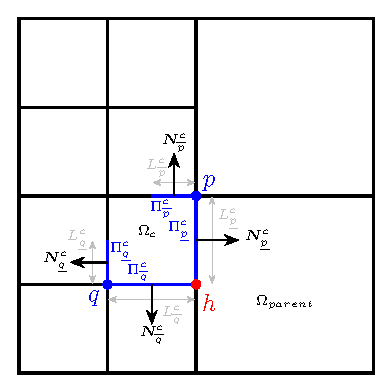
\includegraphics[width=0.48\textwidth]{figure2_reconstructed.pdf}
 \caption{Local kinematics and nodal flux closure at a non-conforming interface. The nodes $p$ and $q$ are independent, whereas $h$ is a geometrically dependent hanging point. For the child cell $c$, the complete segments $ph$ and $qh$ contribute through the nodal pressures $\Pi_{\underline p}^{c}$ and $\Pi_{\overline q}^{c}$, respectively, and no nodal pressure is associated with $h$. The other two highlighted portions retain the standard half-edge contributions $\Pi_{\overline p}^{c}$ and $\Pi_{\underline q}^{c}$.}
 \label{fig:hanging_node_schematic}
\end{figure}

The present construction assumes that the supporting endpoints of every hanging point are independent nodes and that each elementary boundary segment has at least one independent endpoint. Segments with two dependent endpoints and constraints supported by dependent endpoints are outside the present scope. Physical boundary nodes are treated as independent nodes, with their prescribed boundary conditions retained. Under these assumptions, the complete boundary of every cell can be represented using only nodal pressures associated with independent nodes, and the corresponding boundary contributions are formalized next.

\subsection{Cell-edge flux closure without hanging-point pressure}
\label{sec:closure_partition}

The kinematic constraint~\eqref{eq:U_h_constrained} fixes where a hanging point moves, but not how its segments enter the fluxes; that is the task of the closure rule developed here. Each elementary segment of the baseline scheme carries a single half-Riemann relation, built from the cell state and one endpoint node. A segment ending at a hanging point therefore has exactly one relation available---that of its independent endpoint---and the pressure of that endpoint must act over the complete segment: a shorter length would leave part of the boundary unclosed, and a second pressure would require data that $h$ does not carry. Subcell forces then keep the baseline two-term form~\eqref{eq:Fcp}, and only the pressure-action lengths change: the complete segments enter with their full lengths from the outset, as illustrated in Fig.~\ref{fig:hanging_node_schematic}, and no pressure is first evaluated at $h$ and then redistributed.

The directional labels $\overline p$ and $\underline p$ are those of the baseline scheme and serve only to distinguish the two edge directions; they do not imply that the pressure acts over half of the edge. Accordingly, $L_{\overline p}^c$ and $L_{\underline p}^c$ denote the actual pressure-action lengths---a half-segment when both endpoints are independent, the complete segment when the other endpoint is a hanging point---and $\boldsymbol N_{\overline p}^c$, $\boldsymbol N_{\underline p}^c$ the corresponding cell outward unit normals.

The subcell pressures entering~\eqref{eq:Fcp} are given by the baseline linearized half-Riemann relations~\eqref{eq:acoustic}, unchanged: for either portion $s\in\{\overline p,\underline p\}$ of the boundary of cell $c$,
\begin{equation}
 P_c-\Pi_{s}^{c}=Z_c\bigl(\boldsymbol U_p-\boldsymbol U_c\bigr)\cdot\boldsymbol N_{s}^{c},
 \qquad Z_c=\rho_c a_c>0.
 \label{eq:closure_acoustic}
\end{equation}
Equation~\eqref{eq:closure_acoustic} is the baseline relation applied to the complete segment: it couples the cell state to the endpoint velocity alone, and the pressure enters only as the metric weight $\int\Pi\,\boldsymbol N\,dL=\Pi L\boldsymbol N$. That single relation closes the segment: in Fig.~\ref{fig:hanging_node_schematic}, $\Pi_{\underline p}^{c}$ on $ph$ is determined by $\boldsymbol U_p$, whereas $\Pi_{\overline q}^{c}$ on $qh$ is determined by $\boldsymbol U_q$, and no half-Riemann relation or nodal pressure is introduced at $h$.

The contribution of cell $c$ to the balance at node $p$ is
\begin{equation}
 \boldsymbol F_{pc}
 =\Pi_{\overline p}^{c}L_{\overline p}^{c}\boldsymbol N_{\overline p}^{c}
  +\Pi_{\underline p}^{c}L_{\underline p}^{c}\boldsymbol N_{\underline p}^{c}.
 \label{eq:closure_force}
\end{equation}
This is the same two-term expression as in the baseline scheme~\eqref{eq:Fcp}; the non-conforming closure changes nothing but the pressure-action lengths. The nodal force balance~\eqref{eq:momentum_Pi} extends to every independent node $p\in\mathcal P$, the sum over $c\in\mathcal C(p)$ being built from the same pressure-action lengths, and no balance is assembled at a hanging point. Likewise, the semi-discrete system~\eqref{eq:semidiscrete}--\eqref{eq:kinematic} carries over with the boundary sums taken over $\mathcal P(c)$.

The non-conforming closure changes the baseline scheme in one respect only: the pressure-action length of a segment ending at a hanging point becomes the complete segment instead of a half-edge. Three consequences follow. (i) The volume and energy updates use the same endpoint velocity as the pressure, so the segmentwise fluxes match across the interface and the GCL of the coarse cell---the parent of the four children---is preserved; the GCL of an individual child is not, the volume flux over a segment ending at $h$ being evaluated with $\boldsymbol U_p$ alone while the segment moves with both of its endpoints---a discrepancy of $\tfrac12(\boldsymbol U_p-\boldsymbol U_h)\cdot\boldsymbol N\,|ph|$ per segment. (ii) Across a coarse--fine segment the two cell states supply two different nodal pressures, so the interface exchanges momentum through the assembled nodal force balance. (iii) The nodal unknowns, the half-Riemann relations, and the nodal force balances are exactly those of the conforming scheme restricted to independent nodes, so the discretization gains no degree of freedom at $h$.


\subsection{Nodal solver}
\label{sec:closure_solver}

Section~\ref{sec:closure_partition} has specified the subcell pressures and their pressure-action lengths; it remains to determine the nodal velocities. This is achieved exactly as in the baseline scheme: a nodal force balance is assembled at every independent node, and the half-Riemann relations turn it into a linear system for the nodal velocity. No equation is assembled at a hanging point. At an interface node, $\mathcal C(p)$ simply gathers the cells of both resolutions sharing $p$.

Substituting the half-Riemann relations~\eqref{eq:closure_acoustic} into the nodal force balance~\eqref{eq:momentum_Pi} written at $p\in\mathcal P$ and solving for the velocity yields
\begin{equation}
 \boldsymbol U_p=\mathsf M_p^{-1}\sum_{c\in\mathcal C(p)}
 \bigl(\mathsf M_p^c\boldsymbol U_c+P_cL_p^c\boldsymbol N_p^c\bigr),
 \label{eq:closure_solver}
\end{equation}
identical in form to~\eqref{eq:nodalsolver}: the corner vectors and subcell matrices of~\eqref{eq:matrixP} are built from the pressure-action lengths of Section~\ref{sec:closure_partition}, so that at a node adjacent to a hanging point the complete segment length replaces the half-edge length. The solver itself is thus unmodified; the non-conforming geometry enters only through the metric data $L$ and $\boldsymbol N$.

The subcell matrices of~\eqref{eq:matrixP} keep their form under the non-conforming closure, with the pressure-action lengths of Section~\ref{sec:closure_partition} in place of the half-edge lengths; for the projected half-Riemann relations~\eqref{eq:closure_acoustic}, the positive-definiteness argument of Section~\ref{sec:cch} therefore applies verbatim, and $\boldsymbol U_p$ is uniquely determined at every independent node.

Once the independent velocities are known, the hanging-point velocities follow from the constraint~\eqref{eq:U_h_constrained} by direct evaluation---a projection, not a coupled solve. The interface solver is thus a two-stage, iteration-free procedure: solve the baseline nodal system at the independent nodes, then project onto the constraints. No quantity is ever evaluated at a hanging point, and the cost is that of the baseline scheme on the independent nodes alone.

Two conservation properties follow at once from this assembly:
\begin{subequations}
\begin{align}
	\sum_c m_c\,\frac{d\boldsymbol U_c}{dt}
	&=-\sum_{p\in\mathcal P}\sum_{c\in\mathcal C(p)}\boldsymbol F_{pc}=\boldsymbol 0,
	\label{eq:closure_mom}\\
	\sum_c m_c\,\frac{dE_c}{dt}
	&=-\sum_{p\in\mathcal P}\boldsymbol U_p\cdot\Bigl(\sum_{c\in\mathcal C(p)}\boldsymbol F_{pc}\Bigr)=0.
	\label{eq:closure_energy}
\end{align}
\label{eq:closure_conservation}
\end{subequations}
The inner sums in both identities are the nodal force balances~\eqref{eq:momentum_Pi}, which the solver satisfies by construction, and the power in the second is paired with the velocity of the same node, as prescribed in Section~\ref{sec:closure_partition}. Discrete momentum is therefore conserved globally, and the total energy exactly; the entropy inequality carries a remainder on cells with hanging segments and is discussed in the remark of Section~\ref{sec:transfer}.

%% ======================================================================
%  SECTIONS 3.4--3.6 (added this revision; new text in red):
%    3.4  Conservative inter-level transfer and mesh management
%         (p4est, transfers, child-volume check, child-GCL remark)
%    3.5  Solution procedure (time step, Algorithm 1, discrete conservation)
%% ======================================================================

%% (Section 3.4 "Time integration" removed this revision: its step list duplicated
%%  Algorithm 1, and its remaining content was folded into the Solution procedure
%%  section below.)





\subsection{Conservative inter-level transfer and mesh management}
\label{sec:transfer}

The quadtree topology---leaf cells, $2\!:\!1$ balance, ghost layers, and partition across MPI ranks---is managed by \texttt{p4est}~\cite{burstedde2011p4est}; the cell-centred states and the nodal data are stored as payloads on the leaves, and the partition across ranks follows the \texttt{p4est} space-filling-curve (Morton) ordering. The physical operations of the scheme are unaffected by this management: the solvers of Sections~\ref{sec:closure_solver}--\ref{sec:procedure} always act on the current leaf mesh.

\paragraph{Refinement.}
A marked parent is split into four children by exact subdivision---the new nodes are the edge midpoints and the cell centre---so the children stay permanently aligned with the parent and the coarse edges remain straight, and no geometric repair is required. The conserved variables are inherited in proportion to the child volumes $V_i$:
\begin{equation}
	m_i=\frac{V_i}{V_P}\,m_P,\qquad
	(m\boldsymbol U)_i=\frac{V_i}{V_P}\,(m\boldsymbol U)_P,\qquad
	(mE)_i=\frac{V_i}{V_P}\,(mE)_P,
	\label{eq:refine_transfer}
\end{equation}
The children thus share the parent state, and the split carries no projection of physical data. Nodal data need no transfer either: at the next step the independent velocities follow from the local solve on the new leaf mesh, and the hanging points from the projection~\eqref{eq:U_h_constrained}.

\paragraph{Coarsening.}
When a family is coarsened by the rule of Section~\ref{sec:threshold_calibration}, the four children are merged and the conserved variables are aggregated:
\begin{equation}
	m_P=\sum_{i}m_i,\qquad
	(m\boldsymbol U)_P=\sum_i m_i\boldsymbol U_i,\qquad
	(mE)_P=\sum_i m_i E_i.
	\label{eq:coarsen_transfer}
\end{equation}
Both transfers leave the global sums of mass, momentum, and total energy unchanged---the refine weights sum to one, and the coarsening sums are exact. The coarsening remap is first-order and conservative in $(m,m\boldsymbol U,mE)$ but not in internal energy: the kinetic energy carried by the velocity differences among the children is converted into internal energy, an entropy-producing conversion of the correct sign, as is usual for conservative inter-level transfers in ALE--AMR settings~\cite{anderson2004arbitrary}.

\paragraph{Child-volume check.}
Every refined family is monitored through the relative volume residual
\begin{equation}
	r_P=\frac{\bigl|V_P-\sum_{i}V_i\bigr|}{V_P},
	\label{eq:volume_check}
\end{equation}
and a run is aborted when $r_P>10^{-12}$. The subdivision is exact on a convex parent, where the residual vanishes identically; under the sustained distortion of a Lagrangian calculation, however, a cell may lose convexity---an interior angle exceeding $180^\circ$---and the children then fail to partition their parent: some may reverse orientation or overlap, and the child areas no longer sum to the parent area. The check measures precisely this breakdown: it is a geometric failure, not a rounding artifact, and its growth tracks the onset of concavity.

\par\medskip\noindent\textbf{Remark (the child-level GCL mismatch).}
The GCL is satisfied when the face velocity equals the average of the endpoint velocities~\cite{maire2009high}. This condition holds on every edge of the parent of a refined family and fails in a child only on the segments ending at a hanging point, so the mismatch is confined to the interior of the family---and is independent of the check above, being structural, present already in exact arithmetic. Its possible consequence concerns the internal energy of a child, through the entropy balance, and two mechanisms limit it. At refinement the children inherit the state of their parent, so the mismatch arises within a family whose pressures are still equal; and while the family differentiates, the mismatch, being a difference of volume rates, remains under the volume-change restriction of Eq.~\eqref{eq:cfl}. The internal energy remained positive in all calculations reported in Section~\ref{sec:numerics}.

\subsection{Solution procedure}
\label{sec:procedure}

Algorithm~\ref{alg:amr_step} assembles the complete adaptive cycle: an explicit Lagrangian step of Section~\ref{sec:closure_solver} on the current leaf mesh, followed---every $N_{\mathrm{remesh}}$ steps, with $N_{\mathrm{remesh}}=4$ in every calculation reported below---by the marking of Section~\ref{sec:threshold_calibration} and the balancing, transfer, and rebuild of Section~\ref{sec:transfer}. The nodal solve is confined to the independent nodes, the hanging-point projection is a direct evaluation, and the transfers are local to the marked families; the only global operations are the time-step reduction and the norming of the sensors.

\paragraph{Time step.}
The step size is predicted at the beginning of each step from the current state, cell by cell, and reduced to the global minimum over all cells and all ranks. It obeys a CFL condition, a volume-change constraint, and a growth limit,
\begin{equation}
	\Delta t^n\le C_{\mathrm{CFL}}\,\frac{h_c}{a_c},
	\qquad
	\Delta t^n\le \frac{C_v}{\bigl|dV_c^n/dt\bigr|},
	\label{eq:cfl}
\end{equation}
with $h_c$ the shortest edge of the cell, $a_c$ its sound speed, $C_{\mathrm{CFL}}=0.25$ and $C_v=0.01$. Both constants were fixed once for all runs; the volume-change constraint is the binding one wherever the flow converges strongly---on Noh it, rather than the acoustic CFL, sets the step near the origin.

The cell state is advanced by the forward Euler discretisation of~\eqref{eq:mom_evol}--\eqref{eq:ene_evol}, the force and the velocity of the power term being taken at the same time level:
\begin{equation}
	m_c\bigl(\boldsymbol U_c^{n+1}-\boldsymbol U_c^n\bigr)+\Delta t^n\sum_{p\in\mathcal P(c)}\boldsymbol F_{pc}^n=\boldsymbol 0,
	\qquad
	m_c\bigl(E_c^{n+1}-E_c^n\bigr)+\Delta t^n\sum_{p\in\mathcal P(c)}\boldsymbol F_{pc}^n\cdot\boldsymbol U_p^n=0.
	\label{eq:fe_update}
\end{equation}

\par\medskip\refstepcounter{algorithm}%
\noindent\rule{\linewidth}{0.9pt}
\par\noindent\textbf{Algorithm \thealgorithm: one adaptive step of the scheme.}\label{alg:amr_step}
\par\noindent\rule{\linewidth}{0.4pt}
\par\smallskip
\begin{enumerate}\setlength{\itemsep}{1pt}
	\item Compute $\Delta t^n$ from the CFL, volume-change, and growth limits above.
	\item Assemble the pressure-action lengths and normals from $\boldsymbol X^n$ (Section~\ref{sec:closure_partition}).
	\item Solve $\boldsymbol U_p^n$ at every independent node $p\in\mathcal P$ \ (Eq.~\eqref{eq:closure_solver}).
	\item Project $\boldsymbol U_h^n=\tfrac12(\boldsymbol U_{p_1(h)}^n+\boldsymbol U_{p_2(h)}^n)$ for all $h\in\mathcal H$ \ (Eq.~\eqref{eq:U_h_constrained}).
	\item Update $\boldsymbol U_c^{n+1}$ and $E_c^{n+1}$ \ (Eq.~\eqref{eq:fe_update}).
	\item Set $\boldsymbol X^{n+1}=\boldsymbol X^n+\Delta t^n\boldsymbol U^n$; recompute $V_c^{n+1}$, $\rho_c^{n+1}=m_c/V_c^{n+1}$, and $P_c^{n+1}$ from the EOS.
	\item If $(n+1)\bmod N_{\mathrm{remesh}}=0$:
	\begin{enumerate}\setlength{\itemsep}{1pt}
		\item evaluate the sensors $S_c$, $C_c$ and mark with hysteresis and family aggregation \ (Section~\ref{sec:threshold_calibration});
		\item enforce the $2\!:\!1$ balance and build the new leaf topology;
		\item check $r_P\le10^{-12}$ on every refined family \ (Eq.~\eqref{eq:volume_check});
		\item transfer $(m,m\boldsymbol U,mE)$ \ (Eqs.~\eqref{eq:refine_transfer}--\eqref{eq:coarsen_transfer});
		\item rebuild the connectivity and ghost layers; project the hanging points onto the coarse edges.
	\end{enumerate}
\end{enumerate}
\noindent\rule{\linewidth}{0.9pt}
\medskip

The density is thus determined by the geometric volume, and the discrete volume equation~\eqref{eq:vol_evol} is not used to update the thermodynamic state; its status on refined cells is discussed in Section~\ref{sec:closure_partition}.

\subsubsection{Discrete conservation}

Summing the updates~\eqref{eq:fe_update} over all cells and exchanging the order of summation yields
\begin{equation}
	\sum_c m_c\bigl(\boldsymbol U_c^{n+1}-\boldsymbol U_c^n\bigr)
	=-\Delta t^n\sum_{p\in\mathcal P}\Bigl(\sum_{c\in\mathcal C(p)}\boldsymbol F_{pc}^n\Bigr)=\boldsymbol 0,
	\label{eq:fd_mom}
\end{equation}
\begin{equation}
	\sum_c m_c\bigl(E_c^{n+1}-E_c^n\bigr)
	=-\Delta t^n\sum_{p\in\mathcal P}\boldsymbol U_p^n\cdot\Bigl(\sum_{c\in\mathcal C(p)}\boldsymbol F_{pc}^n\Bigr)=0.
	\label{eq:fd_energy}
\end{equation}
The bracketed sums are the nodal force balances at time $t^n$, which the nodal solver satisfies by construction, and the power is paired with the velocity of the same instant---the fully discrete counterpart of the semi-discrete pairing of Section~\ref{sec:closure_solver}. On a closed domain both identities are exact; with reflective boundaries the boundary nodes have zero normal velocity, the boundary forces do no work, and~\eqref{eq:fd_energy} survives unchanged, while the total momentum is balanced by the wall reaction, as it must be. Steps that change the topology interpolate nothing: the transfer operators of Section~\ref{sec:transfer} redistribute $(m,m\boldsymbol U,mE)$ exactly, so the global sums are carried across adaptation without alteration. Both identities are algebraic properties of the scheme and are confirmed numerically to round-off in Section~\ref{sec:numerics_conservation}.

\section{The AMR criteria}
\label{sec:indicator}

The criterion follows one principle: refinement and coarsening are governed by density and pressure gradients. These two fields capture every structure of interest, as in existing ALE--AMR criteria based on normalized solution differences~\cite{anderson2004arbitrary,morrell2007cell}, edge-wise normalized gradients~\cite{waltz2018coupled}, or second-order reconstruction errors~\cite{colaitis2026cell}. The threshold is deliberately generous, keeping the criterion robust without problem-specific tuning. The cost is that weak shocks, once smeared by the capture scheme, may fall below the threshold and escape refinement. Velocity divergence---the operator behind artificial viscosity since von Neumann and Richtmyer~\cite{vonneumann1950method}---is retained as a supplement to protect these structures. We present the gradient criterion first, then its divergence supplement.

\subsection{A gradient criterion on density and pressure}
\label{sec:indicator_thermo}

The strength of a discontinuity is measured by the ratio of the states across it, not by their difference; the latter would couple the threshold to the magnitude of the states themselves. We therefore build the indicator on the logarithms of density and pressure,
\begin{equation}
	q_{\rho,c}=\ln\bigl(\rho_c+\rho_*(c)\bigr),\qquad
	q_{p,c}=\ln\bigl(p_c+p_*(c)\bigr),
	\label{eq:logvars}
\end{equation}
so that their difference recovers the logarithm of the ratio. To avoid degenerate logarithms, the star value is set as:
\begin{equation}
	\rho_*(c)=\varepsilon\rho_{\max}^{\mathrm{glob}},
	\label{eq:regularisation}
\end{equation}
with \(p_*(c)\) defined analogously, \(\varepsilon\) a vacuum bound set to be \(10^{-4}\).

With density and pressure in logarithmic form, the decision rests on a conventional gradient criterion. The gradient of \(q_s\) at cell \(c\) follows from a distance-weighted least-squares fit over the neighbourhood---one equation per neighbour for the two components of \(\nabla q_s\):
\begin{equation}
	\nabla q_{s,c}=\arg\min\sum_{J\in\mathcal{N}(c)}
	\Bigl(\frac{q_{s,J}-q_{s,c}-\nabla q_{s,c}\cdot
		\left(\mathbf{x}_J-\mathbf{x}_c\right)}
	{|\mathbf{x}_J-\mathbf{x}_c|}\Bigr)^{2}.
	\label{eq:lsq}
\end{equation}
This least-squares reconstruction is classical; see~\cite{maire2009high}. The indicator value of a single field is the change of \(q_s\) across the cell,
\begin{equation}
	S_{s,c}=h_c\,M_{s,c},\qquad M_{s,c}=|\nabla q_{s,c}|,
	\label{eq:scdef}
\end{equation}
with \(h_c=\sqrt{V_c}\) the characteristic length. For a jump of total log strength \(\Delta q\) smeared over the \(m\) finest-level cells of the band, the fitted slope reproduces the mean slope and
\begin{equation}
	M_{s,c} \approx \frac{\Delta q}{m\,h_c},
	\qquad\text{hence}\qquad
	S_{s,c} \approx \frac{\Delta q}{m}.
	\label{eq:scappro}
\end{equation}
The reading of a front is thus a relative change per cell: the logarithmic variables render the criterion dimensionless, so the threshold that follows carries no problem-specific physical scale.

Density and pressure are both retained because they respond to different structures: a shock leaves a signature in both, whereas a contact appears in density alone. Their contributions are combined through a root-mean-square sum,
\begin{equation}
	S_c=h_c\sqrt{\bigl(M_{\rho,c}\bigr)^{2}
		+\bigl(M_{p,c}\bigr)^{2}},
	\label{eq:scw}
\end{equation}
so that a single responding field suffices to trigger refinement, while simultaneous responses are combined without doubling. The criterion of this section then reads
\begin{equation}
	\begin{aligned}
		\text{refine } c \text{ if }\ & S_c>\tau_c,\\
		\text{coarsen } P \text{ if }\ & S_{c_i}<\alpha\,\tau_{c_i}\ \text{ for every child } c_i\in P,
	\end{aligned}
	\label{eq:thermo_criteria}
\end{equation}
with \(\alpha\in[0,1]\) the ratio of the coarsening threshold to the refinement threshold.




\subsection{A Velocity-Divergence Supplement to the AMR Criterion}
\label{sec:indicator_kinematic}
\label{sec:threshold_calibration}

A generous threshold has a price: a weak shock, smeared by the capture scheme over
several cells, may carry a gradient below \(\tau_c\) and be left to the numerical
dissipation. Such a structure is a compression, and compression carries a direct
signal on a moving mesh.

The velocity divergence---the detector behind artificial viscosity since von
Neumann and Richtmyer~\cite{vonneumann1950method}---supplies it. On a moving mesh
it is the relative rate of volume change, evaluated in boundary form as the flux
of the mesh motion through the faces of the cell,
\begin{equation}
	F_c=\sum_{f\subset\partial\Omega_c}L_f\,\tfrac12\bigl(\boldsymbol{U}_a+\boldsymbol{U}_b\bigr)\cdot\boldsymbol{N}_f,
	\label{eq:fk}
\end{equation}
with the same averaged face velocity that moves the mesh
(Eq.~\eqref{eq:vol_evol}).

Measured against the volume rate \(h_c\,u_{\max}\) swept across the cell, where $u_{\max}$ is the global maximum nodal speed of the current mesh state---the maximum of \(|\boldsymbol U|\) over all cell centroids and cell corners, reduced to one value across ranks and recomputed once per step---and truncated to its compressive part, this flux
gives the dimensionless compression rate
\begin{equation}
	C_c=\frac{\max(-F_c,0)}{h_c\,u_{\max}},
	\label{eq:ck}
\end{equation}
the fraction of the cell volume compressed per crossing---order one at a shock and
vanishing for smooth expansion---and bounded by \(1/m\) for a shock smeared over
\(m\) cells. For comparison, the velocity term of Cola{\"i}tis
et al.~\cite{colaitis2026cell} is a velocity gradient, whereas here it is the
divergence, which measures the compression itself.

The supplement completes the criterion, with its own threshold \(\mu_c\) and the same
hysteresis ratio \(\alpha\):
\begin{equation}
	\begin{aligned}
		\text{refine } c \text{ if }\ & S_c>\tau_c \ \text{ or }\ C_c>\mu_c,\\
		\text{coarsen } P \text{ if }\ & S_{c_i}<\alpha\,\tau_{c_i} \ \text{ and }\ C_{c_i}<\alpha\,\mu_{c_i}\ \text{ for every child } c_i\in P.
	\end{aligned}
	\label{eq:criteria}
\end{equation}
A cell is refined as soon as either part responds, while a family is coarsened only
when every child falls below both thresholds.




%% ======================================================================
%  SECTION 5: ACCURACY ON FIXED-TOPOLOGY NON-CONFORMING MESHES
%% ======================================================================
\section{Accuracy on fixed-topology non-conforming meshes}
\label{sec:tgv_convergence}

Fixing the mesh topology isolates the interface treatment from the remeshing errors examined in Section~\ref{sec:numerics}: the mesh is refined once before the first hydrodynamic update and is then advected with the flow, so any departure from the exact solution is due to the closure described in Section~\ref{sec:hanging_solver}, rather than inter-level transfer. The Taylor--Green vortex~\cite{dobrev2012high} serves as the accuracy benchmark: it is smooth and admits an exact steady solution, so the formal order of the discretization can be measured without a reference calculation.

The flow is posed on the unit square $\Omega=[0,1]\times[0,1]$ with wall boundaries and an ideal gas with adiabatic index $\gamma=1.4$. The initial state is
\begin{equation}
	u_0=\sin(\pi x)\cos(\pi y),\qquad v_0=-\cos(\pi x)\sin(\pi y),\qquad \rho_0=1,\qquad P_0=\tfrac14\bigl[\cos(2\pi x)+\cos(2\pi y)\bigr]+1,
	\label{eq:tgv_ic}
\end{equation}
This state is an exact steady solution: the velocity field is divergence-free and the pressure gradient balances the convective term, so the density and the specific internal energy remain constant in time. For this test case only, a source term is added to the internal-energy update so that the same state satisfies the discrete energy balance:
\begin{equation}
	\overline{s}_e=\frac{5\pi}{8}\Bigl[\cos(\pi x)\cos(3\pi y)-\cos(3\pi x)\cos(\pi y)\Bigr],
	\label{eq:tgv_source}
\end{equation}
Because this forcing is non-conservative, the Taylor--Green case does not test global energy conservation.

Four meshes with base levels $L=4,\dots,7$ are used. In each mesh, base cells whose radial intervals intersect the annulus $0.1\le r\le0.4$ about the center $(0.5,0.5)$ are refined by one level; the topology is then frozen, and no further adaptation is performed. All runs are advanced to $t=0.6$. The cell velocity $\boldsymbol U_c$ is compared with the exact field $\boldsymbol u_0$ at the cell centroid $\boldsymbol x_c$ in the $L_2$ norm
\begin{equation}
	\|e_u\|_{L_2}=\Bigl(\sum_c\bigl|\boldsymbol U_c-\boldsymbol u_0(\boldsymbol x_c)\bigr|^{2}A_c\Bigr)^{1/2},
	\qquad \sum_c A_c=|\Omega|=1,
	\label{eq:tgv_l2}
\end{equation}
where the sum runs over leaf cells and $A_c$ is the cell area; the effective mesh size reported in Table~\ref{tab:tgv_convergence} is $h_{\mathrm{eff}}=\sqrt{|\Omega|/N}$.

\begin{table}[pos=htbp]
	\centering
	\caption{Grid convergence of the Taylor--Green vortex at $t=0.6$ on fixed-topology non-conforming meshes. The error is the $L_2$ velocity norm of Eq.~\eqref{eq:tgv_l2} against the exact steady field; the order is measured using $h_{\mathrm{eff}}$.}
	\label{tab:tgv_convergence}
	\begin{tabular}{lcccc}
		\hline
		Mesh & $N$ & $h_{\mathrm{eff}}$ & $\|e_u\|_{L_2}$ & Order \\
		\hline
		Levels 4--5 & 736   & $3.69\times10^{-2}$ & $2.48\times10^{-1}$ & ---  \\
		Levels 5--6 & 2656  & $1.94\times10^{-2}$ & $1.46\times10^{-1}$ & 0.83 \\
		Levels 6--7 & 10324 & $9.8\times10^{-3}$  & $7.78\times10^{-2}$ & 0.92 \\
		Levels 7--8 & 40408 & $5.0\times10^{-3}$  & $4.06\times10^{-2}$ & 0.95 \\
		\hline
	\end{tabular}
\end{table}

The error decreases monotonically, and the observed order increases from $0.83$ to $0.95$, approaching the first-order rate of the explicit scheme. The time step is not an independent parameter here: with the CFL and volume-change constraints of Eq.~\eqref{eq:cfl}, the step is controlled by the coarsest cells of the mesh and changes very little across the four hierarchies (mean $\Delta t=1.46\times10^{-4}$, $1.46\times10^{-4}$, $1.46\times10^{-4}$ and $1.36\times10^{-4}$ from Levels 4--5 to 7--8, a variation of seven percent while $h_{\mathrm{eff}}$ falls by a factor of $7.4$). A temporal error component would therefore be nearly constant across the sequence, while the error itself falls by $6.1$; the measured orders are thus set by the spatial discretisation. A complete separation of the two would require rescaling $\Delta t$ with the mesh, which is not attempted here. Figure~\ref{fig:tgv_velocity} shows the velocity magnitude at the final time for the four meshes, using a common color scale with the mesh overlaid. The steady vortex is reproduced at every level, the level interfaces leave no visible trace in the contours, and the flow structure is insensitive to distortion of the rotating core cells; the flux closure remains reliable as the non-conforming mesh is refined.

\begin{figure}[pos=htbp]
	\centering
	\begin{subfigure}{0.47\textwidth}
		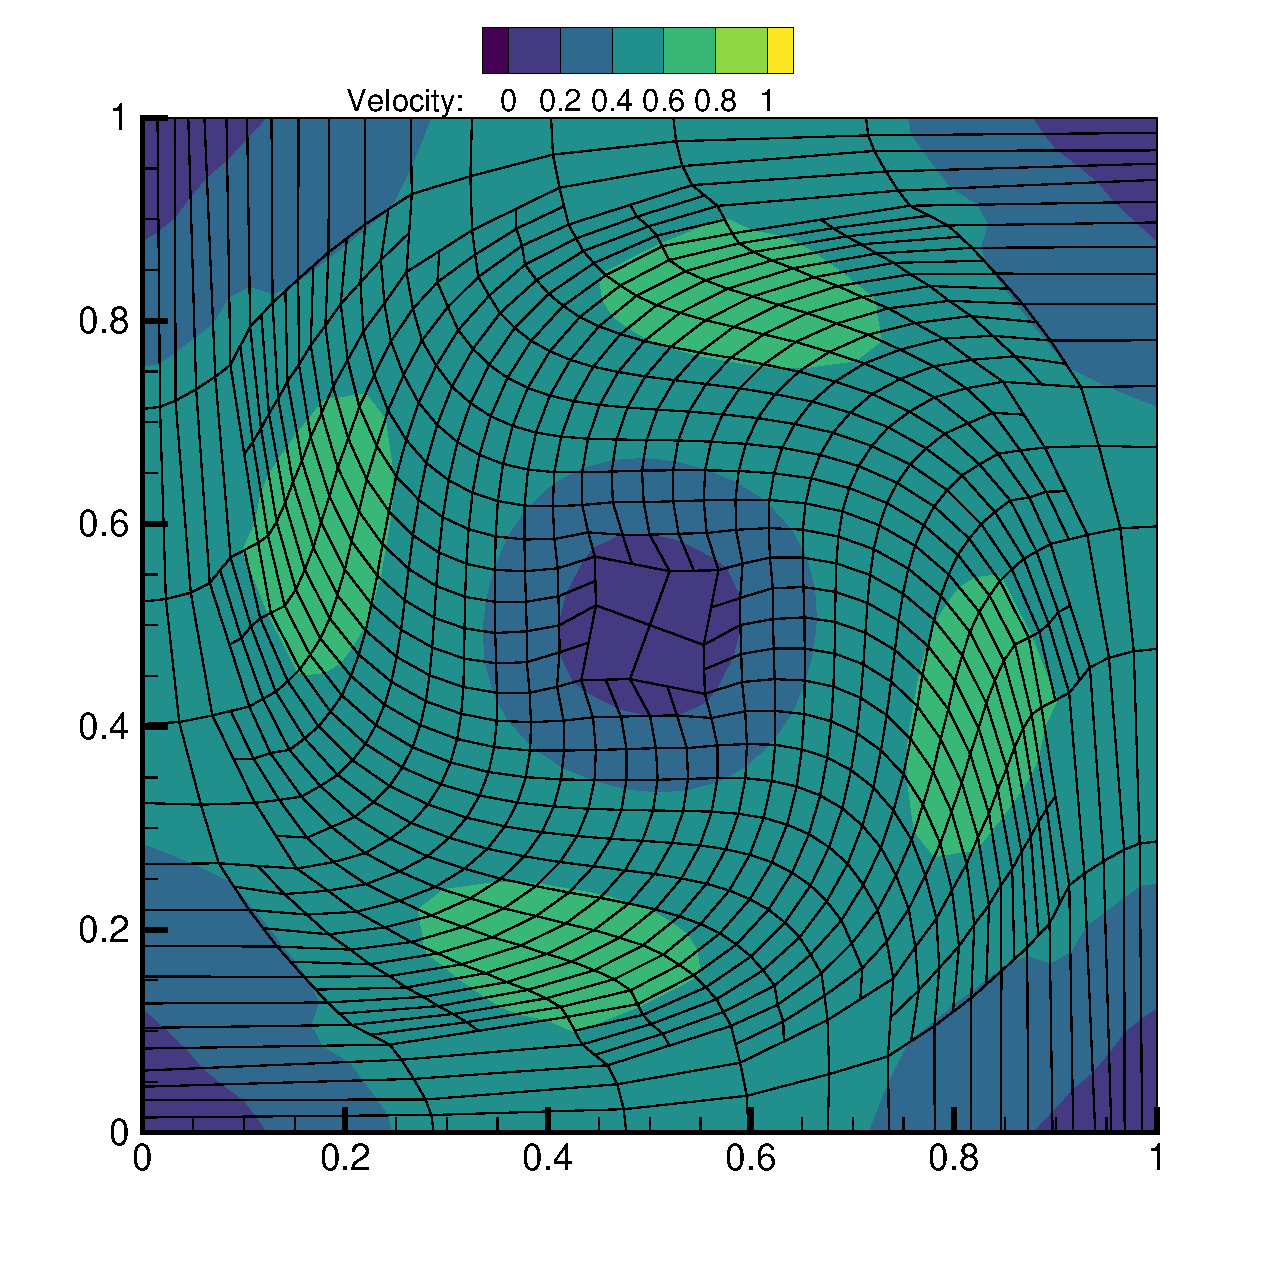
\includegraphics[width=\linewidth]{results/taylor-green/taylor-green-l4-5-velocity-contour}
		\caption{Levels 4--5}
	\end{subfigure}\hfill
	\begin{subfigure}{0.47\textwidth}
		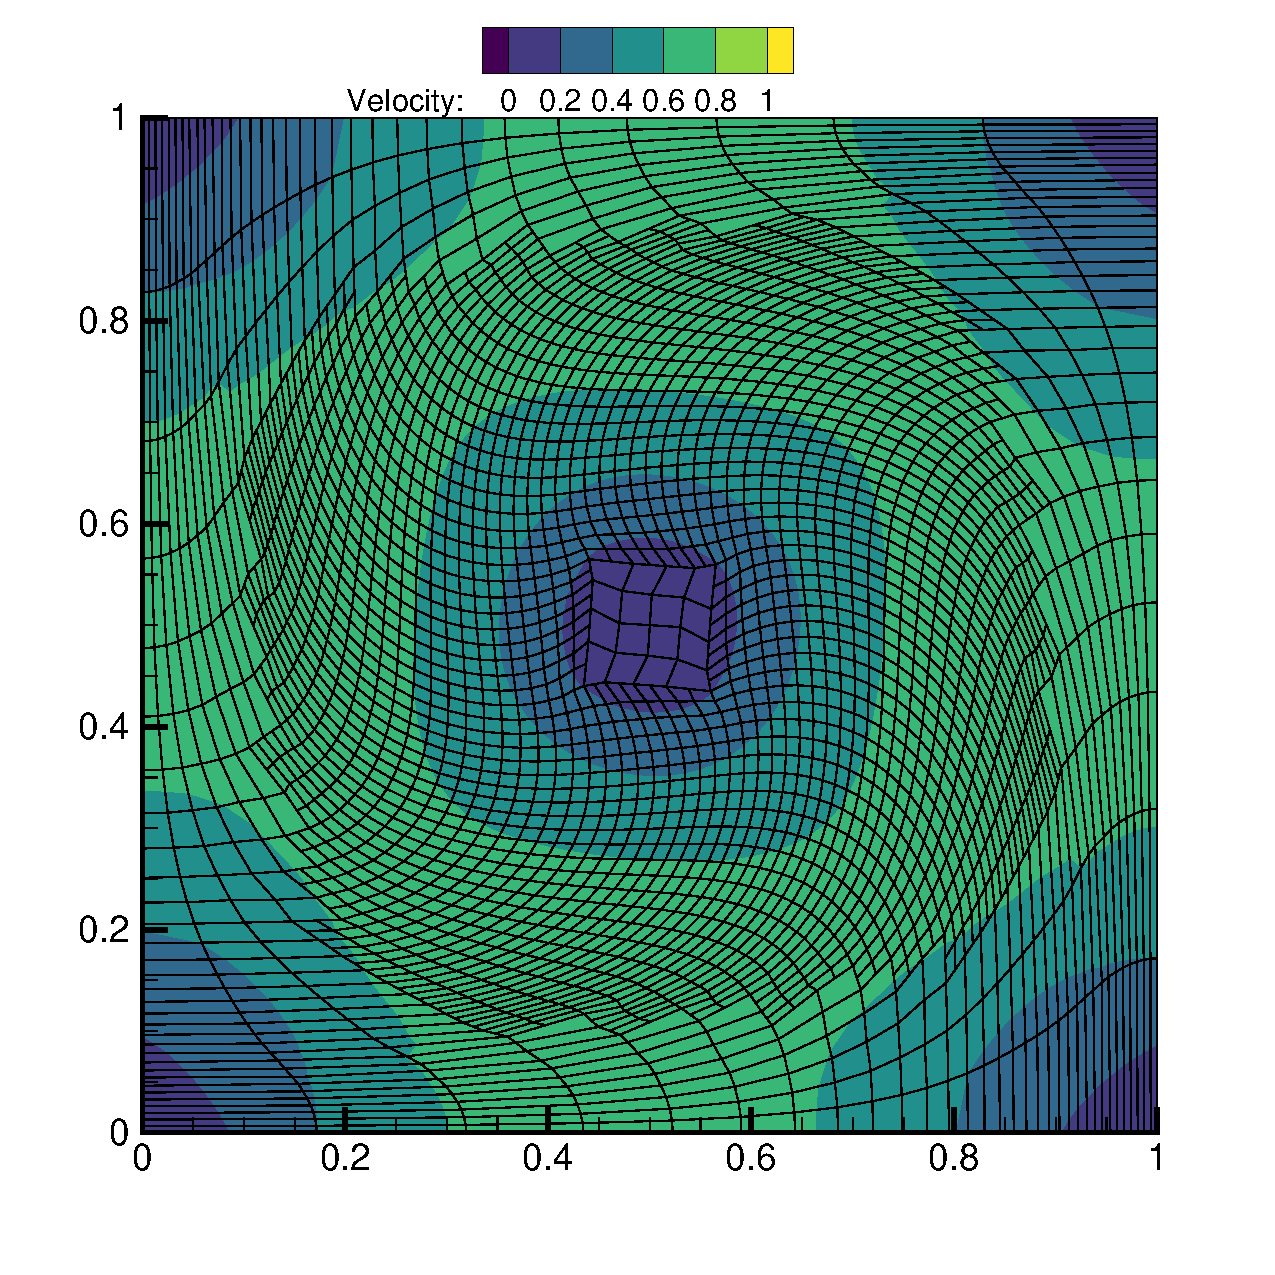
\includegraphics[width=\linewidth]{results/taylor-green/taylor-green-l5-6-velocity-contour}
		\caption{Levels 5--6}
	\end{subfigure}
	\\[4pt]
	\begin{subfigure}{0.47\textwidth}
		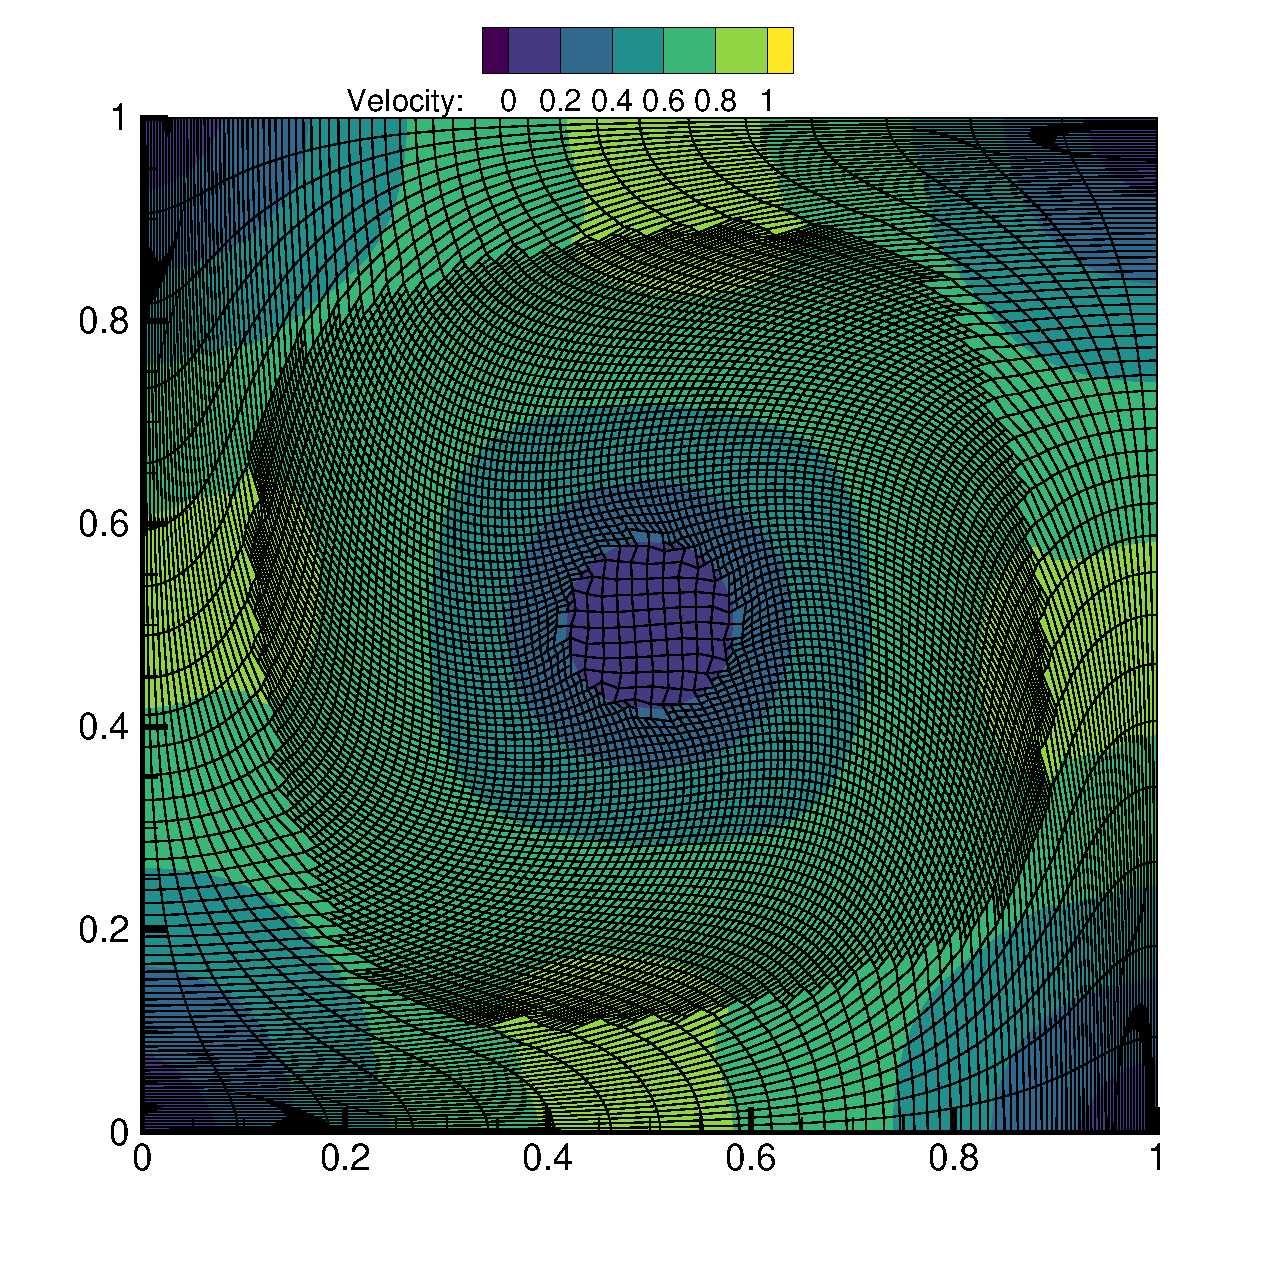
\includegraphics[width=\linewidth]{results/taylor-green/taylor-green-l6-7-velocity-contour}
		\caption{Levels 6--7}
	\end{subfigure}\hfill
	\begin{subfigure}{0.47\textwidth}
		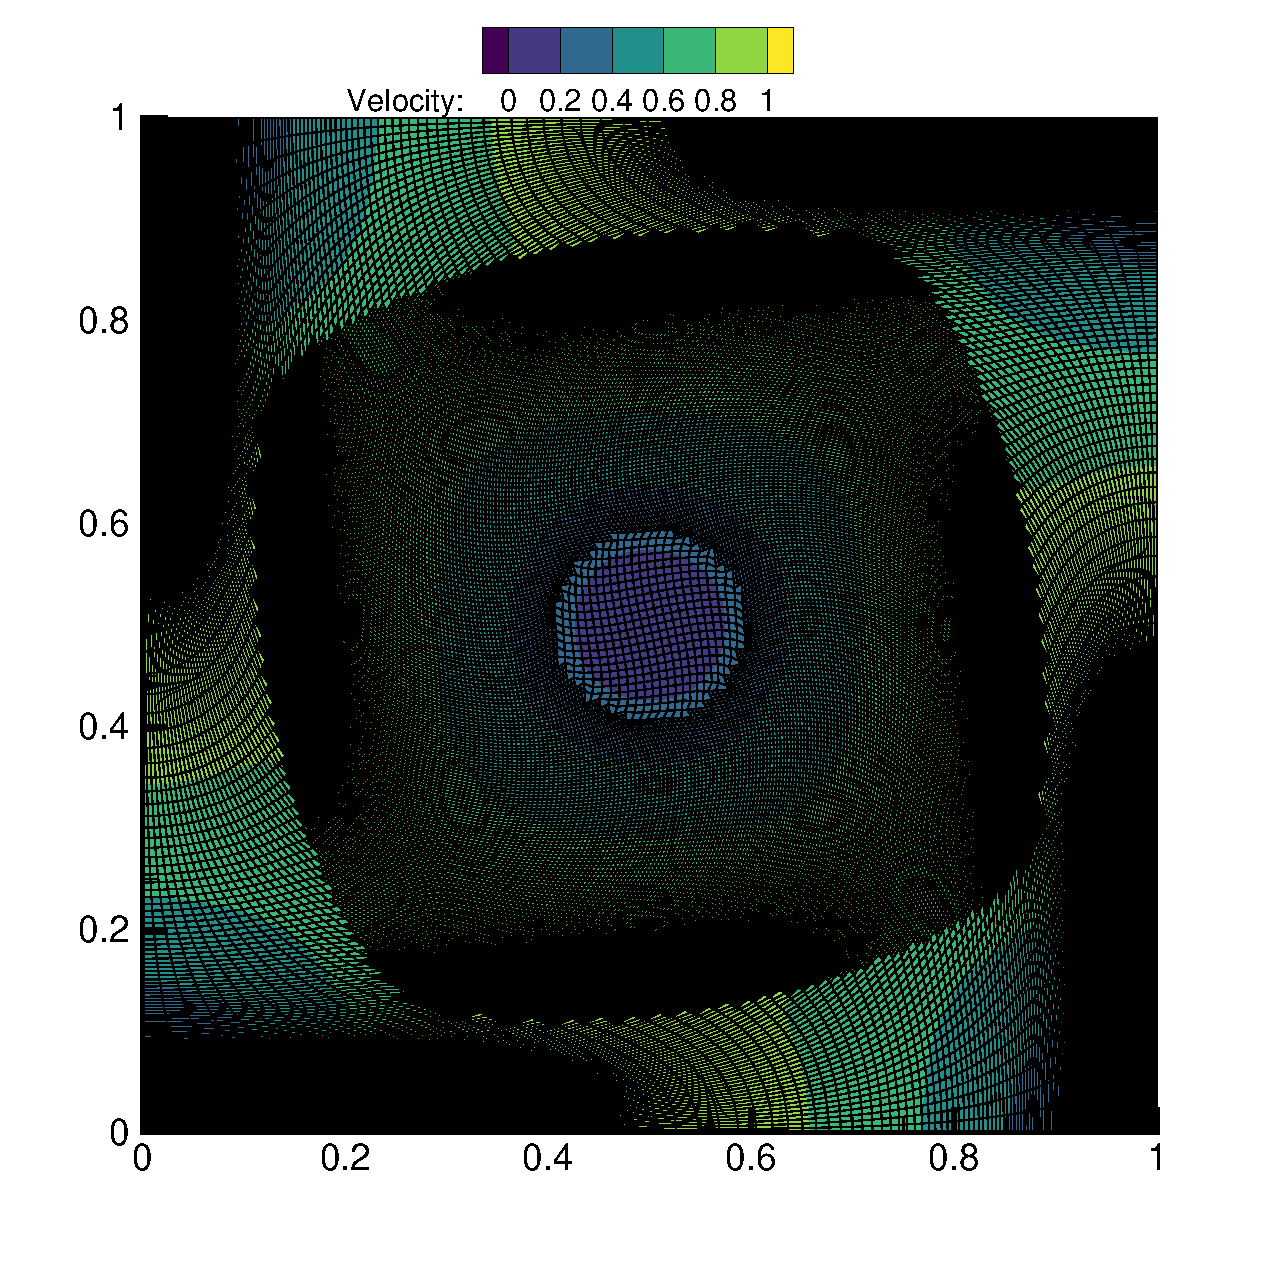
\includegraphics[width=\linewidth]{results/taylor-green/taylor-green-l7-8-velocity-contour}
		\caption{Levels 7--8}
	\end{subfigure}
	\caption{Magnitude of the velocity field, $|\boldsymbol U|$, at the final time $t=0.6$ on the fixed-topology non-conforming meshes of Table~\ref{tab:tgv_convergence}, using a common color scale with the mesh overlaid. Base cells intersecting the annulus $0.1\le r\le0.4$ about the center $(0.5,0.5)$ are refined once, and the topology is then frozen; the mesh is carried by the flow, so the rotating-core cells become distorted by the final time.}
	\label{fig:tgv_velocity}
\end{figure}

% TODO (authors): four final-time mesh plots, for Levels 4--5 to 7--8, remain to be inserted
%   after Figure~\ref{fig:tgv_velocity}.

%% ======================================================================
%  SECTION 6: NUMERICAL ASSESSMENT
%  Data status: eta=0.75 series and Tensor-dissipation@0.30/0.225 are in
%  (Tables hysteresis / level_noh).  Still pending: pre-failure
%  energy drift, uniform-reference wall-clock, load-balance metrics.
%% ======================================================================
\section{Numerical assessment of the refinement strategy}
\label{sec:numerics}

This section validates the statements of Section~\ref{sec:indicator} on three classical shock problems and documents the conservation and efficiency of the adaptive calculations. Each subsection opens with the property it verifies.
All calculations were performed on a single desktop node with an Intel Core i5-10210U processor (four cores, eight threads, $1.60$\,GHz base frequency) and $16$\,GB of memory; every run, uniform and adaptive alike, uses four MPI ranks on this node, one per physical core. All runs stem from one code, produced as a small number of builds of the same lineage whose differences are confined to experimental AMR toggles---the hydrodynamic core, and with it every conservation property of Section~\ref{sec:procedure}, is identical---and the Noh tables use a single build throughout. Cell counts and widths are unaffected by the build; CPU times agree between builds to roughly ten percent, and the speed-ups are accordingly read as order-of-magnitude figures. No parallel-scaling study is reported: the fixed four-rank configuration serves only to make the quoted wall-clock times mutually comparable. % TODO: code version (compiler + optimization level)

The refinement thresholds, fixed once for all problems and levels, follow the calibration of Section~\ref{sec:threshold_calibration} and are listed in Table~\ref{tab:amr_parameters}. With $S_c\approx \ln(R)/m$ from Eq.~\eqref{eq:scappro}, we find that $\tau_c=0.5$ already captures all fronts in the tests below without tuning, while remaining well above smooth gradients. Similarly, with $C_c\le 1/m$ from Eq.~\eqref{eq:ck}, a shock over three cells reads at most $1/3$, so $\mu_c=0.2$ stays below this ceiling and above smooth compression. The supplement study of Section~\ref{sec:compression} additionally probes the more sensitive value $\mu_c=0.05$, which the weak shocks of the Sod fan require; every run states its operative $\mu_c$ in its table caption. The hysteresis ratio $\alpha=0.75$ avoids irreversible refinement at $\alpha\to0$ and refinement--coarsening cycling at $\alpha\to1$.

\begin{table}[pos=htbp]
	\centering
	\caption{Thresholds of the refinement criterion of Section~\ref{sec:indicator}, fixed once for all calculations of Section~\ref{sec:numerics}. The supplement study of Section~\ref{sec:compression} lowers the compression threshold to $\mu_c=0.05$, as required by the weak Sod shock; the operative tuple of every run is restated in its table caption.}
	\label{tab:amr_parameters}
	\begin{tabular}{lll}
		\hline
		Parameter & Value & Rationale \\
		\hline
		Thermodynamic threshold $\tau_c$ & $0.5$ & captures all test shocks, well above smooth gradients \\
		Hysteresis ratio $\alpha$ & $0.75$ & avoids irreversible refinement ($\alpha\to0$) and cycling ($\alpha\to1$) \\
		Compression threshold $\mu_c$ & $0.2$ & below the $1/3$ ceiling for a shock over $3$ cells, above smooth compression \\
		\hline
	\end{tabular}
\end{table}


\subsection{Setup and error metrics}
\label{sec:numerics_metrics}

Three classical shock problems are computed on quarter domains with symmetry conditions on the coordinate axes; the assessment is confined to single-material ideal-gas flows, and beyond the radial symmetry of these problems the mesh-motion stress on the closure is exercised by the rotating core of the frozen-topology vortex of Section~\ref{sec:tgv_convergence}. The \emph{Sedov blast wave}~\cite{sedov1959similarity,kamm2007efficient} is posed on $[0,1.2]^2$ with free outflow on the outer boundaries: a cold gas at rest, $\gamma=1.4$, $\rho_0=1$, $e_0=10^{-5}$, with a total internal energy of $0.244816$ deposited in the cell adjacent to the origin at $t=0$. The self-similar solution carries the front outward to \(r\approx1.0\) at \(t=1\), with a post-shock density peak of \(\rho=6.0\). The \emph{Noh problem}~\cite{noh1987errors} is posed on the unit square: a cold gas, $\gamma=5/3$, $\rho_0=1$, $P_0=10^{-6}$, converging onto the origin with the unit-speed radial inflow $\boldsymbol U_0=-\boldsymbol x/|\boldsymbol x|$; the exact solution carries the front at $r=t/3$ with the post-shock plateau $\rho=16$. The \emph{Sod shock tube}~\cite{sod1978survey} is posed in cylindrical symmetry on the unit square with reflective boundaries, the initial discontinuity at $r=0.5$ separating $(\rho,P)=(1,1)$ inside from $(0.125,0.1)$ outside, the gas at rest, $\gamma=5/3$.
% TODO: reconcile the ambient values against the run scripts before submission
%   (Sedov e_0=1e-5 -> P_0=4e-6 for gamma=1.4; Noh P_0=1e-6).

Accuracy is assessed at the final state, unless stated otherwise, through four quantities. \emph{(i)~Shock physical width:} let $\rho_L$ and $\rho_R$ be the densities just behind and ahead of the shock. Two threshold pairs are used. In the \emph{fixed} pair, $\rho_L$ and $\rho_R$ are the analytic values where available (Sedov: $6$ and $1$; Noh: $\rho_L=16$ with $\rho_R=3.85$ taken from the finest uniform run); in the \emph{adaptive} pair $\rho_L$ is replaced by the run's own post-shock peak, so that coarse meshes, whose peak is smeared below the analytic value, remain measurable. Along each of $90$ radial rays (one per degree in the quarter domain), walk inward and locate the radii at which the density crosses
\begin{equation}
	\rho_{20}=\rho_L+0.2\,(\rho_R-\rho_L),\qquad \rho_{80}=\rho_L+0.8\,(\rho_R-\rho_L),
	\label{eq:wthresh}
\end{equation}
linearly interpolating between the two adjacent cells that straddle each threshold, and take
\begin{equation}
	W_{\mathrm{shock}}=r_{80}-r_{20}.
	\label{eq:wshock}
\end{equation}
The 20\%/80\% percentiles keep the reading away from the peak tip of a strong shock, whose height varies between meshes, and measuring ray by ray and reporting the median removes any dependence on the order in which cells are traversed. A ray whose peak does not reach $\rho_{20}$ is counted as \emph{unresolved}. A uniformly refined sequence should narrow $W_{\mathrm{shock}}$ in proportion to the mesh size, and an adaptive run that refines at the front should reach the width of the uniformly refined reference at its finest level. \emph{(ii)~Refinement coverage:} the percentage of the cells inside the shock band $[r_{20},r_{80}]$ of the adaptive run \emph{itself} that lie at its finest level. The band is thus self-referential: the coverage states that the refinement sits on the transition the run actually resolves, not that this transition already matches the uniform width---the two part company when the captured front still carries the memory of an earlier, coarser stage (the Noh discussion of Section~\ref{sec:sedov} exhibits exactly this case). \emph{(iii)~Cost:} CPU time and the speed-up against the uniformly refined run at the finest level. \emph{(iv)~Conservation:} the maximum relative drift of the discrete total energy,
\begin{equation}
	\varepsilon_E=\max_t\frac{\bigl|\sum_c m_cE_c(t)-\sum_cm_cE_c(0)\bigr|}{\sum_cm_cE_c(0)},
	\label{eq:edrift}
\end{equation}
including the inter-level transfers of Section~\ref{sec:transfer} on the adaptive runs.


\subsection{Sedov and Noh problems with the gradient criterion}
\label{sec:sedov}

Both problems are computed with the gradient criterion of
Section~\ref{sec:indicator_thermo} alone---the thermodynamic channel without
the divergence supplement of Section~\ref{sec:threshold_calibration}---so the
two subsections that follow assess the criterion in its pure form.

\paragraph{Shock width and refinement coverage.}
Tables~\ref{tab:sedov_shock} and~\ref{tab:noh_shock} collect the shock
physical width of Eq.~\eqref{eq:wshock}, the fraction of the shock band
covered by the finest level, the cell-steps, the CPU time and its speed-up
against the uniformly refined run at the finest level, and the maximum
energy drift, for the uniform grids L4--L8 and the adaptive hierarchies. On
both problems the uniformly refined sequence narrows the captured shock
monotonically, in proportion to the mesh size---on Sedov from
$W_{\mathrm{shock}}=0.041$ (L5) down to $0.0020$ (L8), on Noh from $0.041$
(L5) down to $0.0032$ (L8)---and the fixed and adaptive threshold pairs give
nearly the same widths, so the sequence does not depend on which pair is
used. The L4 runs are \emph{unresolved}: their peak density never reaches
$\rho_{20}$. The adaptive runs resolve the shock as narrowly as a much finer
uniform grid, at a fraction of its cost. On Sedov, L4--L7 gives
$W_{\mathrm{shock}}=0.0048$, the width of uniform L7 ($0.0044$), at a
$47\times$ speed-up, and L5--L8 gives $0.0021$, matching uniform L8
($0.0020$), at $20\times$; on Noh, L4--L7 gives $0.0079$, between uniform
L6 and L7, at $87\times$, and L5--L8 gives $0.0036$, within $12\%$ of L8
($0.0032$) and well below uniform L7 ($0.0065$), at $29\times$. The coverage
column confirms the mechanism: $85\%$ and $88\%$ of the Sedov shock band and
$100\%$ of the Noh band are covered by the finest level, so the refinement is
placed precisely on the transition that sets the width.
The two Noh widths nevertheless exceed their uniform counterparts, and the
reason is the history of the front rather than the placement of the
refinement: the Noh shock exists from $t=0$ and sweeps the entire domain, each
hierarchy starts at its base level, and the front is smeared on that coarse
mesh first; since the Lagrangian children inherit the state of their parent,
refinement refines the transition it finds---it cannot reset a transition
already smeared. On Sedov, by contrast, the front is born at the energy
deposition point and outruns its own early smeared stage, so the adaptive
widths match the uniform ones; the residual offset on Noh is the price of the
history, not of the coverage.
Figures~\ref{fig:sedov_l4l7}--\ref{fig:noh_l4l7_enlarge} show the
corresponding level distributions and density fields.

\begin{figure}[pos=htbp]
	\centering
	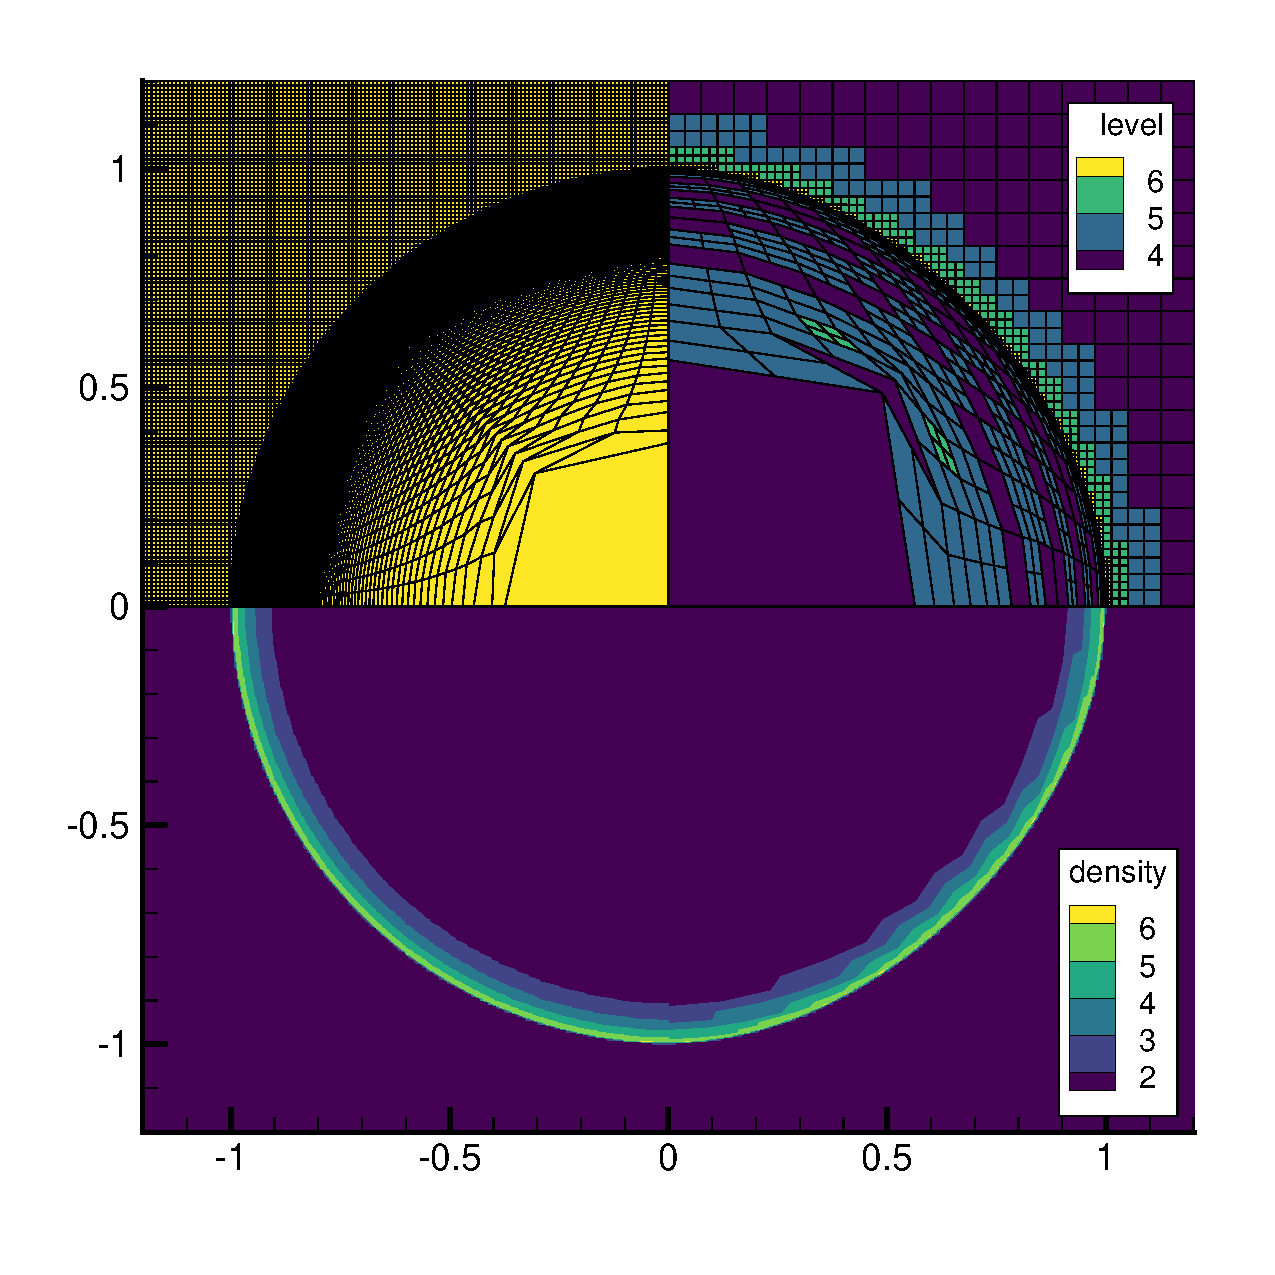
\includegraphics[width=0.8\textwidth]{results1013/sedov/SEDOV-L4-L7.eps}
	\caption{Sedov blast wave at $t=1$, hierarchy L4--L7 vs.\ uniform L7: level distribution (above the $x$ axis) and density contours (below). The refinement collects in a narrow band along the front, and the adaptive front and contours match the uniform reference.}
	\label{fig:sedov_l4l7}
\end{figure}

\begin{figure}[pos=htbp]
	\centering
	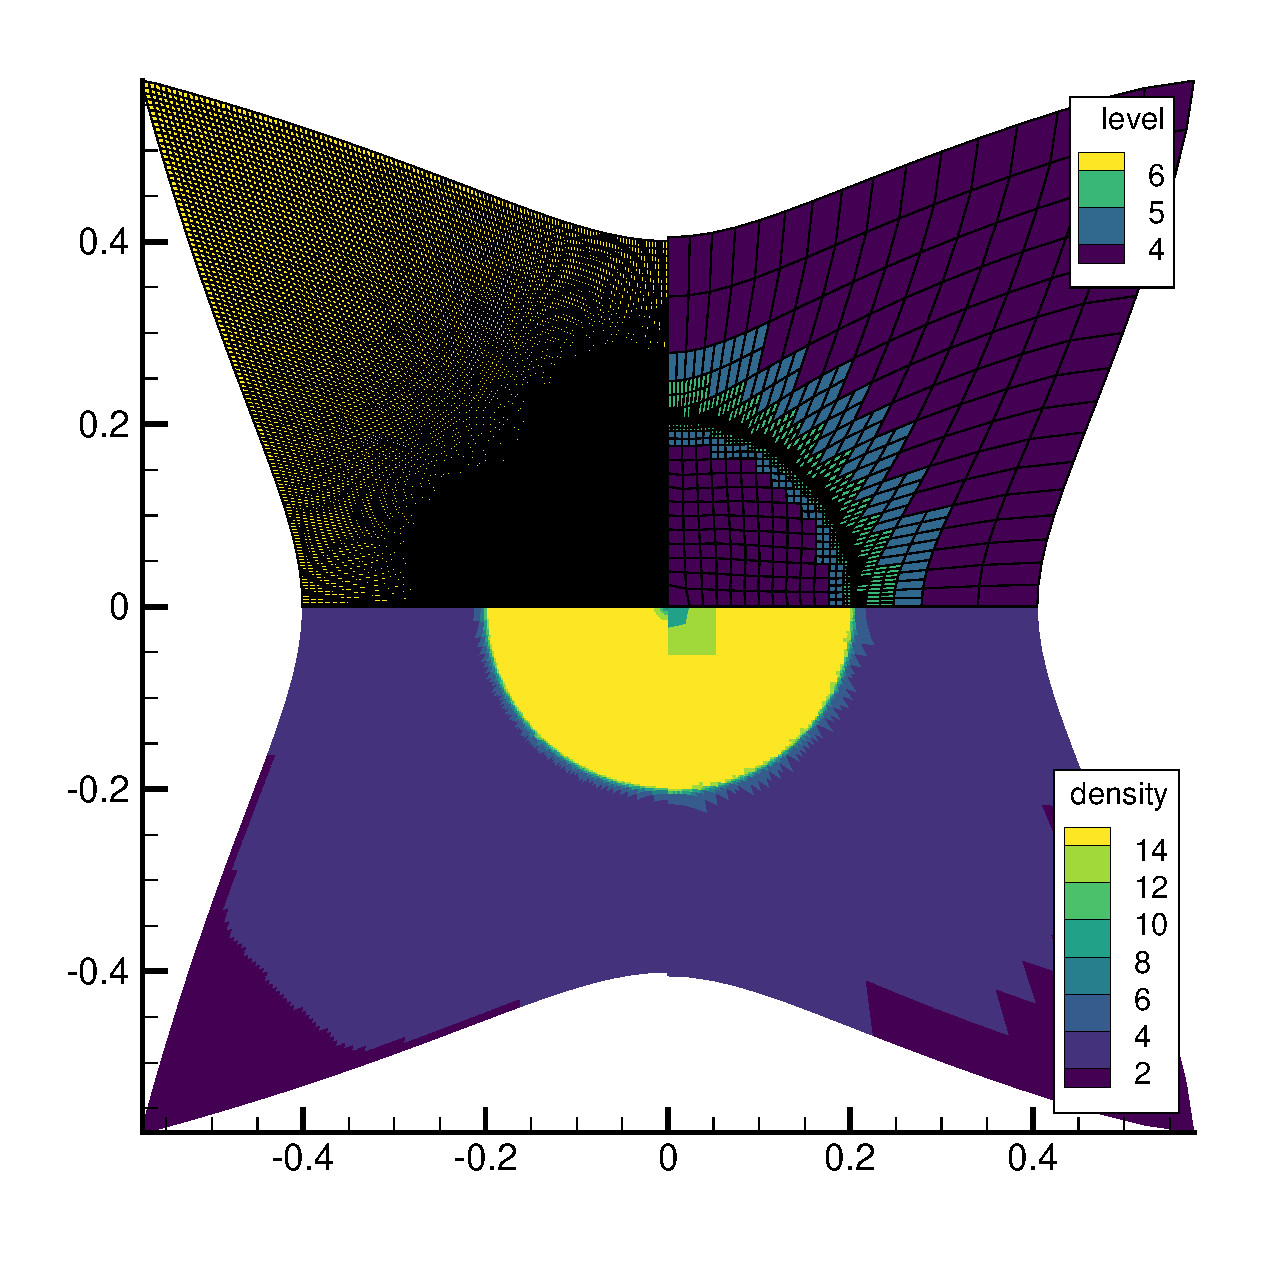
\includegraphics[width=0.8\textwidth]{results1013/noh/noh-L4-L7.eps}
	\caption{Noh problem at $t=0.6$, hierarchy L4--L7 vs.\ uniform L7: level distribution (above the $x$ axis) and density contours (below), in the layout of Figure~\ref{fig:sedov_l4l7}. The refinement covers the shock band, and the adaptive front and post-shock plateau match the uniform reference.}
	\label{fig:noh_l4l7}
\end{figure}

\begin{figure}[pos=htbp]
	\centering
	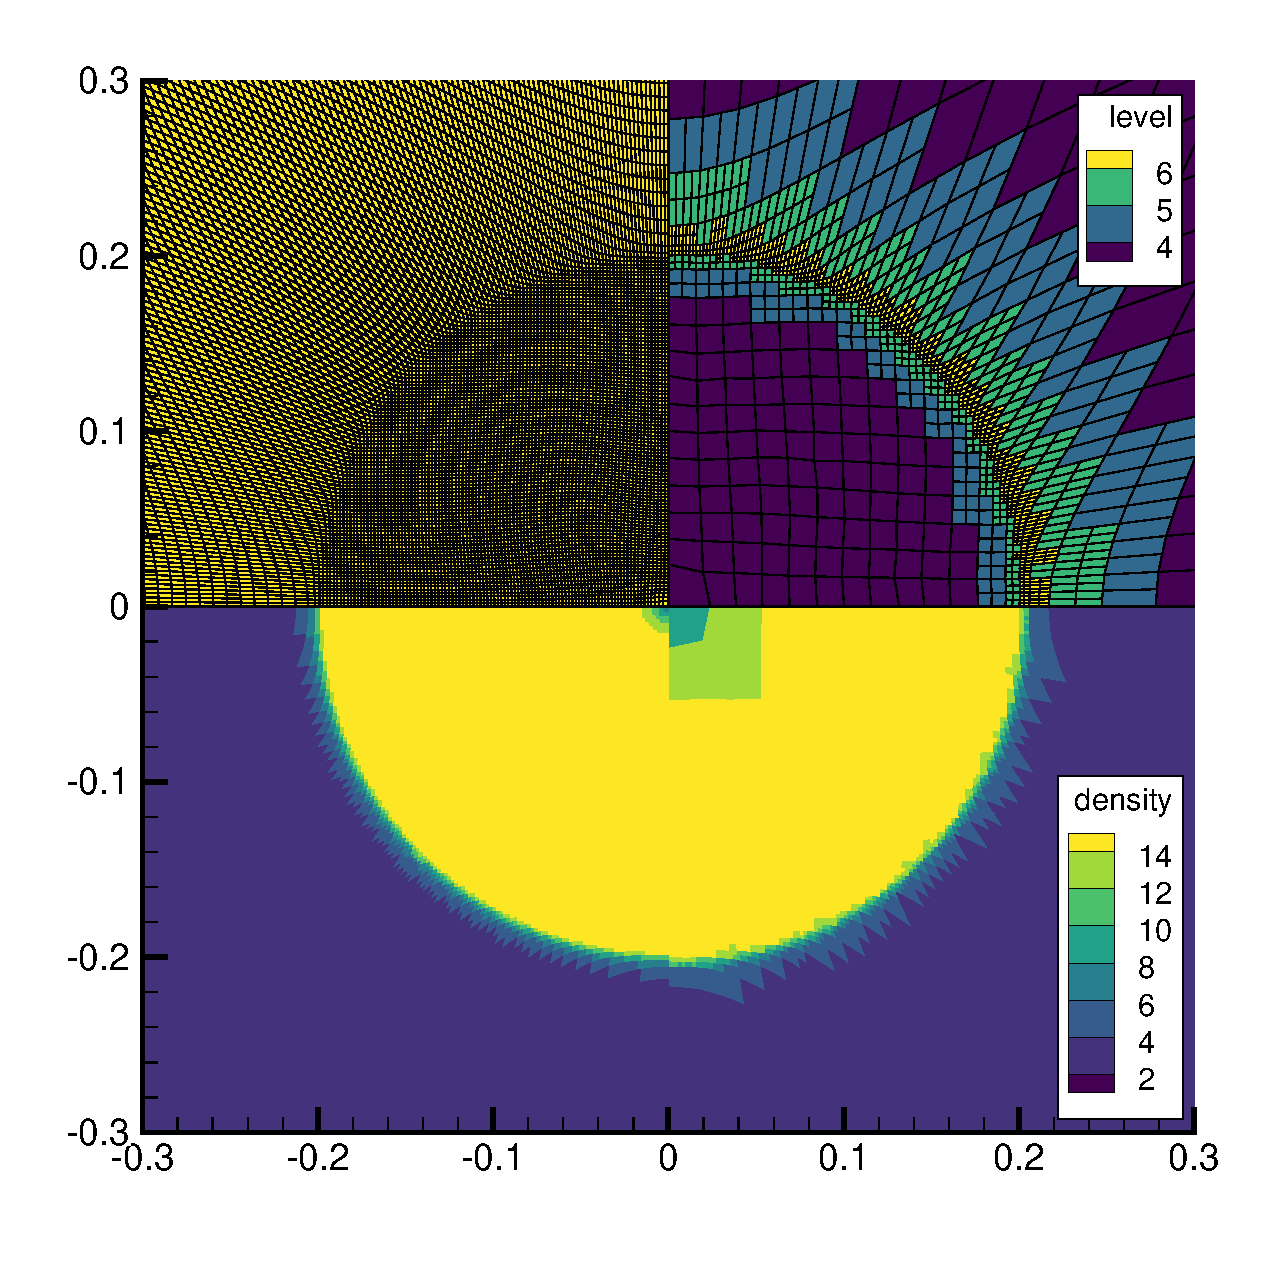
\includegraphics[width=0.8\textwidth]{results1013/noh/noh-L4-L7-enlarge.eps}
	\caption{Enlargement of the shock band of Figure~\ref{fig:noh_l4l7}: the post-shock plateau ring, the smeared transition over the refined cells, and its junction with the coarser interior.}
	\label{fig:noh_l4l7_enlarge}
\end{figure}

\paragraph{Conservation.}
\label{sec:numerics_conservation}
Every run of both problems conserves the total energy to round-off, with
drifts between $1.3\times10^{-15}$ and $5.1\times10^{-13}$
(Tables~\ref{tab:sedov_shock} and~\ref{tab:noh_shock}). The adaptive values,
$\varepsilon_E\le6.0\times10^{-15}$ on Sedov and $\le4.9\times10^{-15}$ on
Noh, include every refinement and coarsening transfer and are among the
smallest in each table: the inter-level transfers of
Section~\ref{sec:transfer} redistribute $(m,m\boldsymbol U,mE)$ exactly and
introduce no conservation error of their own, confirming numerically the
algebraic identities of Section~\ref{sec:procedure}.

\begin{table}[pos=htbp]
	\centering
	\caption{Sedov blast wave at $t=1$: shock physical width
	$W_{\mathrm{shock}}$ of Eq.~\eqref{eq:wshock} for the fixed threshold pair
	($\rho_L=6$, $\rho_R=1$, i.e.\ $\rho_{20}=5.0$, $\rho_{80}=2.0$) and for
	the adaptive pair; the fraction of the shock band $[r_{20},r_{80}]$
	covered by the finest level for the adaptive runs; cell-steps; CPU time
	and its speed-up against the uniform L8 run; and the maximum energy drift
	of Eq.~\eqref{eq:edrift}. \emph{Unresolved} marks runs whose peak density
	does not reach $\rho_{20}$. On this problem the captured shock is only
	about one cell of the finest level wide, so widths differing by less than
	a cell spacing are not distinguishable. All runs use four MPI ranks on
	one node.}
	\label{tab:sedov_shock}
	\begin{tabular}{lccccccc}
		\hline
		Mesh & Cell-steps & $W_{\mathrm{shock}}$ (fixed) & $W_{\mathrm{shock}}$ (adapt.) & Coverage & CPU (s) & Speed-up & $\varepsilon_E$ \\
		\hline
		Uniform L4 ($16^2$)  & $1.18\times10^{6}$ & \emph{unresolved} & $0.0568$ & ---      & $22.1$   & $166\times$  & $6.0\times10^{-15}$ \\
		Uniform L5 ($32^2$)  & $4.73\times10^{6}$ & $0.0409$          & $0.0340$ & ---      & $73.6$   & $50.0\times$ & $4.8\times10^{-15}$ \\
		Uniform L6 ($64^2$)  & $1.89\times10^{7}$ & $0.0109$          & $0.0107$ & ---      & $343.2$  & $10.7\times$ & $6.0\times10^{-14}$ \\
		Uniform L7 ($128^2$) & $7.56\times10^{7}$ & $0.0044$          & $0.0044$ & ---      & $970.2$  & $3.8\times$  & $6.9\times10^{-14}$ \\
		Uniform L8 ($256^2$) & $3.06\times10^{8}$ & $0.0020$          & $0.0022$ & ---      & $3678.0$ & $1\times$    & $5.1\times10^{-13}$ \\
		Adaptive L4--L7      & $3.67\times10^{6}$ & $0.0048$          & $0.0048$ & $85.3\%$ & $77.7$   & $47.3\times$ & $4.8\times10^{-15}$ \\
		Adaptive L5--L8      & $9.21\times10^{6}$ & $0.0021$          & $0.0023$ & $87.5\%$ & $185.1$  & $19.9\times$ & $4.8\times10^{-15}$ \\
		\hline
	\end{tabular}
\end{table}

\begin{table}[pos=htbp]
	\centering
	\caption{Noh problem at $t=0.6$: shock physical width of
	Eq.~\eqref{eq:wshock} for the fixed pair ($\rho_L=16$, $\rho_R=3.85$,
	i.e.\ $\rho_{20}=13.6$, $\rho_{80}=6.28$) and for the adaptive pair, and
	the remaining columns as in Table~\ref{tab:sedov_shock}, the speed-up
	being against the uniform L8 run.}
	\label{tab:noh_shock}
	\begin{tabular}{lccccccc}
		\hline
		Mesh & Cell-steps & $W_{\mathrm{shock}}$ (fixed) & $W_{\mathrm{shock}}$ (adapt.) & Coverage & CPU (s) & Speed-up & $\varepsilon_E$ \\
		\hline
		Uniform L4 ($16^2$)  & $1.05\times10^{6}$ & \emph{unresolved} & $0.0502$ & ---      & $22.9$   & $174\times$  & $1.3\times10^{-15}$ \\
		Uniform L5 ($32^2$)  & $4.21\times10^{6}$ & $0.0406$          & $0.0365$ & ---      & $73.0$   & $54.5\times$ & $4.2\times10^{-15}$ \\
		Uniform L6 ($64^2$)  & $1.68\times10^{7}$ & $0.0144$          & $0.0142$ & ---      & $251.4$  & $15.8\times$ & $4.9\times10^{-15}$ \\
		Uniform L7 ($128^2$) & $6.74\times10^{7}$ & $0.0065$          & $0.0065$ & ---      & $986.7$  & $4.0\times$  & $1.1\times10^{-13}$ \\
		Uniform L8 ($256^2$) & $2.93\times10^{8}$ & $0.0032$          & $0.0032$ & ---      & $3975.2$ & $1\times$    & $3.1\times10^{-13}$ \\
		Adaptive L4--L7      & $2.00\times10^{6}$ & $0.0079$          & $0.0079$ & $100\%$  & $45.6$   & $87.2\times$ & $1.6\times10^{-15}$ \\
		Adaptive L5--L8      & $6.93\times10^{6}$ & $0.0036$          & $0.0037$ & $100\%$  & $135.7$  & $29.3\times$ & $4.9\times10^{-15}$ \\
		\hline
	\end{tabular}
\end{table}

\subsection{Three shock problems with the compression supplement}
\label{sec:compression}

The gradient criterion of Section~\ref{sec:sedov} refines where density and
pressure gradients are largest. On Sedov and Noh this puts the finest level
exactly on the front, but on the Sod wave fan it does not: the fan is wide, and
its weaker structures---the contact and the rarefaction, once smeared---carry
the largest gradients, while the shock itself is left with too few refined
cells. The supplement of Section~\ref{sec:threshold_calibration} adds a
refinement request wherever the flow compresses, independently of the gradient
magnitude. All supplement runs below use the compression threshold
$\mu_c=0.05$---the more sensitive value announced in
Section~\ref{sec:numerics}, required by the weak Sod shock---while the
gradient thresholds $\tau_c$ and $\alpha$ keep the values of
Table~\ref{tab:amr_parameters}; the default $\mu_c=0.2$ serves as the
comparison point on Noh and is quoted in the text. The two subsections below assess it: first on Sod, where the
criterion alone is insufficient, and then on Sedov and Noh, which are
recomputed as a counterpart.

\paragraph{Sod.}
The Sod shock tube is posed in cylindrical symmetry on the unit square, with
the initial discontinuity at $r=0.5$ separating $(\rho,P)=(1,1)$ inside from
$(0.125,0.1)$ outside. Its cylindrical wave fan admits no analytic solution,
so the uniformly refined L8 run serves as the reference.
Table~\ref{tab:sod_compression} shows what the supplement changes. With the
gradient criterion alone the transition is barely resolved: its captured width
is $0.17$--$0.22$, four to eight times that of the supplement runs, it is
detectable on only $1$, $7$ and $78$ of the $90$ rays---elsewhere the peak does
not even reach the upper threshold---no cell of the shock band lies at the
finest level, and the width is not even monotone in the hierarchy. Adding the
compression channel covers the band completely with the finest level and brings
the width down monotonically---$0.0404$ at L3--L6, $0.0201$ at L4--L7 and
$0.0097$ at L5--L8, the last matching the uniform L8 value of $0.0108$---at a
fraction of the cost of uniform refinement: $2.2$, $5.2$ and $12.2$ million
cell-steps and $43$, $94$ and $200$ seconds against $4.9\times10^{8}$
cell-steps and $4385$ seconds at L8, speed-ups of $102$, $47$ and $22$ against
the uniform reference. One remark belongs
here: the widths are measured on the shock, with $\rho_L=0.2055$ and
$\rho_R=0.125$, and because the contact discontinuity of this problem is far
steeper than the shock, the scan starts outside the fan so that the first
crossing taken is the shock.

\begin{table}[pos=htbp]
	\centering
	\caption{Sod problem at $t=0.2$ with the compression supplement: shock
	physical width of Eq.~\eqref{eq:wshock} for the fixed threshold pair
	($\rho_L=0.2055$, $\rho_R=0.125$, i.e.\ $\rho_{20}=0.189$,
	$\rho_{80}=0.141$) and for the adaptive pair, and the remaining columns as
	in Table~\ref{tab:sedov_compression}. The adaptive rows use the supplement
	with $\mu_c=0.05$; $\tau_c=0.5$ and $\alpha=0.75$ as in
	Table~\ref{tab:amr_parameters}. The thresholds are taken on the
	shock; the contact discontinuity, which is the steeper feature of this
	problem, is excluded by starting the scan outside the fan. The
	gradient-only rows measure a transition the gradient criterion has not
	resolved: their widths are detectable on only $1$, $7$ and $78$ of the
	$90$ rays, no cell of the shock band lies at the finest level, and the
	width is not monotone in the hierarchy; those rows are quoted for
	reference, and the speed-up range quoted in the text refers to the
	supplement rows.}
	\label{tab:sod_compression}
	\begin{tabular}{lccccccc}
		\hline
		Mesh & Cell-steps & $W_{\mathrm{shock}}$ (fixed) & $W_{\mathrm{shock}}$ (adapt.) & Coverage & CPU (s) & Speed-up & $\varepsilon_E$ \\
		\hline
		Uniform L3 ($8^2$)   & $1.95\times10^{5}$ & $0.1988$ & $0.1821$ & ---      & $5.8$    & $756\times$   & $1.0\times10^{-15}$ \\
		Uniform L4 ($16^2$)  & $7.80\times10^{5}$ & $0.1213$ & $0.1126$ & ---      & $14.1$   & $311\times$   & $1.8\times10^{-15}$ \\
		Uniform L5 ($32^2$)  & $3.12\times10^{6}$ & $0.0799$ & $0.0739$ & ---      & $51.1$   & $85.8\times$  & $5.7\times10^{-15}$ \\
		Uniform L6 ($64^2$)  & $1.25\times10^{7}$ & $0.0392$ & $0.0391$ & ---      & $177.7$  & $24.7\times$  & $1.7\times10^{-14}$ \\
		Uniform L7 ($128^2$) & $5.23\times10^{7}$ & $0.0206$ & $0.0214$ & ---      & $940.4$  & $4.7\times$   & $6.1\times10^{-14}$ \\
		Uniform L8 ($256^2$) & $4.94\times10^{8}$ & $0.0108$ & $0.0114$ & ---      & $4384.7$ & $1\times$     & $2.1\times10^{-13}$ \\
		L3--L6, gradient only   & $8.25\times10^{5}$ & $0.1744$ & $0.1751$ & $0\%$    & $20.6$   & $213\times$   & $1.8\times10^{-15}$ \\
		L3--L6, with supplement & $2.19\times10^{6}$ & $0.0404$ & $0.0448$ & $100\%$  & $43.1$   & $102\times$   & $3.1\times10^{-15}$ \\
		L4--L7, gradient only   & $1.74\times10^{6}$ & $0.2172$ & $0.1578$ & $0\%$    & $37.6$   & $117\times$   & $3.1\times10^{-15}$ \\
		L4--L7, with supplement & $5.15\times10^{6}$ & $0.0201$ & $0.0214$ & $100\%$  & $94.1$   & $46.6\times$  & $4.4\times10^{-15}$ \\
		L5--L8, gradient only   & $4.82\times10^{6}$ & $0.0815$ & $0.0742$ & $0\%$    & $95.3$   & $46.0\times$  & $5.4\times10^{-15}$ \\
		L5--L8, with supplement & $1.22\times10^{7}$ & $0.0097$ & $0.0105$ & $100\%$  & $200.2$  & $21.9\times$  & $1.0\times10^{-14}$ \\
		\hline
	\end{tabular}
\end{table}

\begin{figure}[pos=htbp]
	\centering
	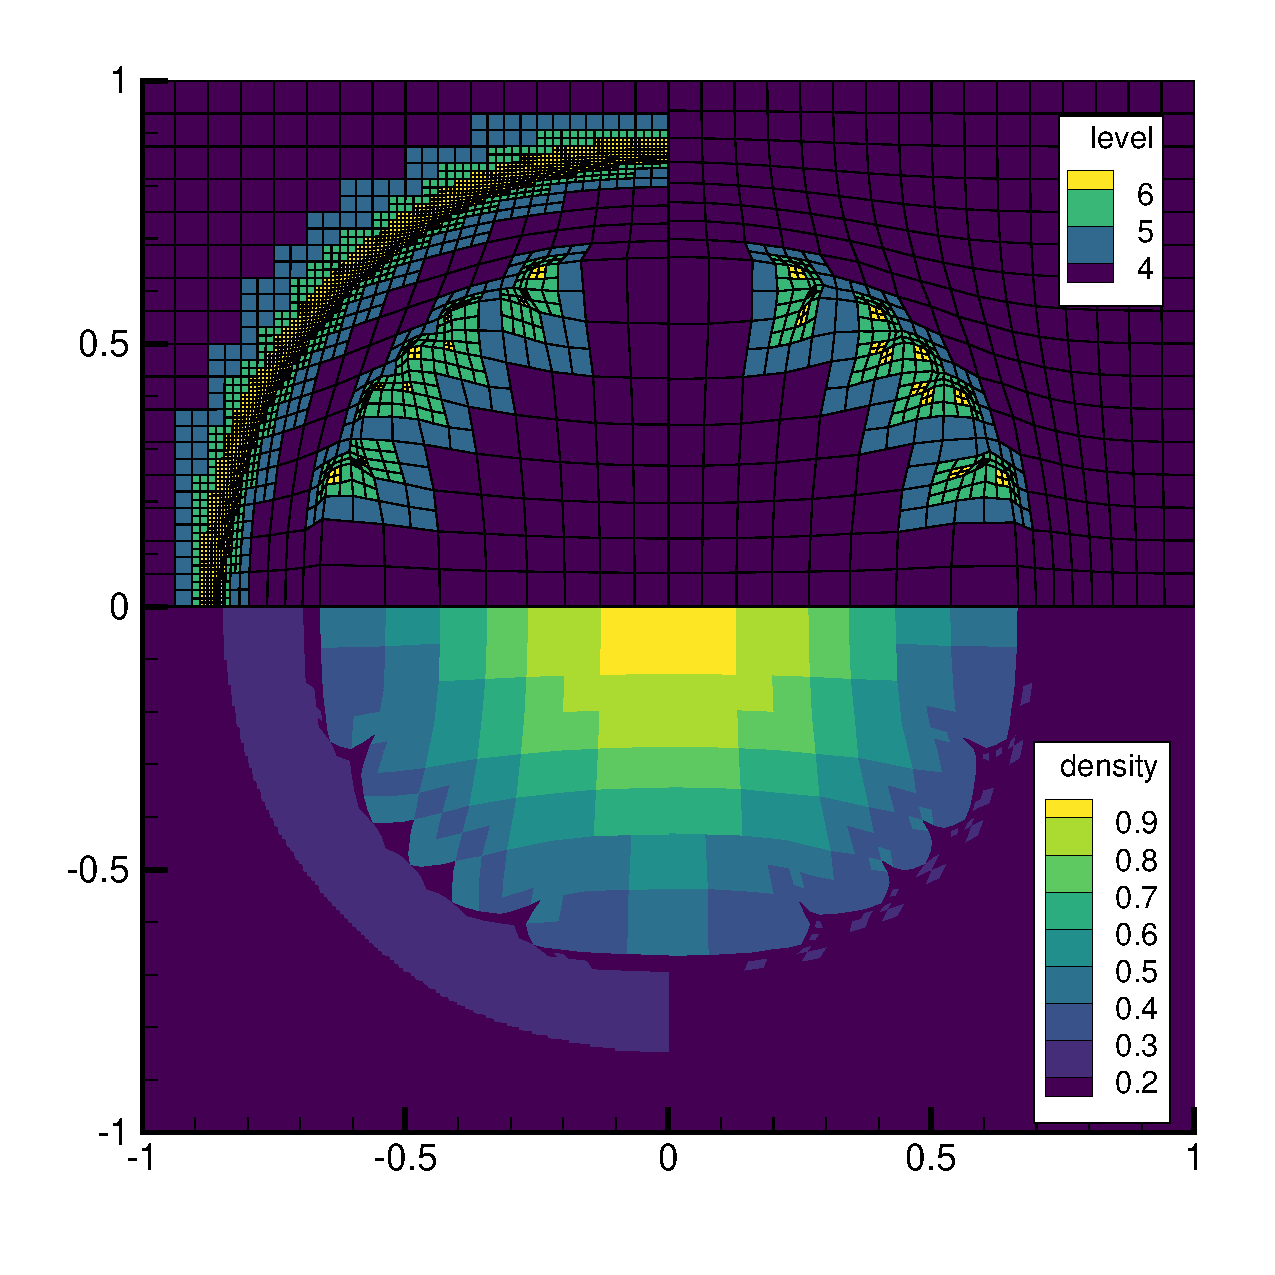
\includegraphics[width=0.8\textwidth]{results1013/sod/sod-l4-l7.eps}
	\caption{Sod problem at $t=0.2$, hierarchy L4--L7, in the layout of Figure~\ref{fig:sedov_l4l7}: level distribution (above the $x$ axis) and density field (below). The refinement collects along the shock, while the smooth interior and the ambient region stay at the coarse levels.}
	\label{fig:sod_l4l7}
\end{figure}

\paragraph{Sedov and Noh.}
On the two problems where the gradient criterion already resolves the front,
the supplement changes little.
Tables~\ref{tab:sedov_compression} and~\ref{tab:noh_compression} compare the
hierarchies L4--L7 and L5--L8 with and without the extra channel, against the
uniform run at their finest level. On Sedov the width is unchanged to within
the resolution of the measurement---$0.0048\to0.0047$ and $0.0021\to0.0020$,
against $0.0044$ and $0.0020$ for uniform L7 and L8---the covered fraction of
the band rises from $85\%$ to $95\%$ on L4--L7, and the cost does not move.
Two supplement rows even read slightly shorter CPU times than their
gradient-only counterparts; the cell-step counts differ by barely one
percent---the added requests concentrate the finest level on a narrower band,
which the coarsening reclaims earlier---while the CPU difference, of order ten
percent, lies within the build-to-build variability noted in
Section~\ref{sec:numerics}. On
Noh the supplement does narrow the shock, from $0.0078$ to $0.0066$ and from
$0.0036$ to $0.0033$, but the cost grows much faster than the gain: L4--L7
goes from $2.0\times10^{6}$ to $1.6\times10^{7}$ cell-steps and from $46$ to
$380$ seconds for a $15\%$ narrower transition, and L5--L8 from
$6.9\times10^{6}$ to $2.3\times10^{7}$ cell-steps and from $136$ to $570$
seconds for $8\%$. A comparison within one code path shows the same
saturation: at $\mu=0.2$ the Noh widths are $0.0072$ and $0.0034$, only about
$8\%$ wider than at $\mu=0.05$, while the cell-steps fall by a factor of three
to six. The supplement is therefore best read as a targeted repair for fronts
that the gradient criterion misses rather than a default refinement channel:
where the criterion already resolves the transition, the extra requests buy
little and cost a great deal.

\begin{table}[pos=htbp]
	\centering
	\caption{Sedov blast wave at $t=1$: shock physical width of
	Eq.~\eqref{eq:wshock} for the fixed threshold pair ($\rho_L=6$, $\rho_R=1$,
	i.e.\ $\rho_{20}=5.0$, $\rho_{80}=2.0$) and for the adaptive pair, for the
	uniform runs at the finest two levels and for the hierarchies L4--L7 and
	L5--L8 computed with the gradient criterion alone and with the compression
	supplement; the fraction of the shock band $[r_{20},r_{80}]$ covered by the
	finest level; cell-steps; CPU time and its speed-up against the uniform L8
	run; and the maximum energy drift of Eq.~\eqref{eq:edrift}. The supplement
	rows use $\mu_c=0.05$; $\tau_c=0.5$ and $\alpha=0.75$ as in
	Table~\ref{tab:amr_parameters}. All runs use
	four MPI ranks on one node.}
	\label{tab:sedov_compression}
	\begin{tabular}{lccccccc}
		\hline
		Mesh & Cell-steps & $W_{\mathrm{shock}}$ (fixed) & $W_{\mathrm{shock}}$ (adapt.) & Coverage & CPU (s) & Speed-up & $\varepsilon_E$ \\
		\hline
		Uniform L7 ($128^2$)    & $7.56\times10^{7}$ & $0.0044$ & $0.0044$ & ---      & $970.2$  & $3.8\times$  & $6.9\times10^{-14}$ \\
		Uniform L8 ($256^2$)    & $3.06\times10^{8}$ & $0.0020$ & $0.0022$ & ---      & $3678.0$ & $1\times$    & $5.1\times10^{-13}$ \\
		L4--L7, gradient only   & $3.67\times10^{6}$ & $0.0048$ & $0.0049$ & $85.3\%$ & $77.7$   & $47.3\times$ & $4.8\times10^{-15}$ \\
		L4--L7, with supplement & $3.63\times10^{6}$ & $0.0047$ & $0.0047$ & $95.4\%$ & $68.9$   & $53.4\times$ & $5.3\times10^{-15}$ \\
		L5--L8, gradient only   & $9.21\times10^{6}$ & $0.0021$ & $0.0023$ & $87.5\%$ & $185.1$  & $19.9\times$ & $4.8\times10^{-15}$ \\
		L5--L8, with supplement & $9.38\times10^{6}$ & $0.0020$ & $0.0022$ & $88.2\%$ & $166.8$  & $22.0\times$ & $7.7\times10^{-15}$ \\
		\hline
	\end{tabular}
\end{table}

\begin{table}[pos=htbp]
	\centering
	\caption{Noh problem at $t=0.6$: shock physical width of
	Eq.~\eqref{eq:wshock} for the fixed pair ($\rho_L=16$, $\rho_R=3.85$,
	i.e.\ $\rho_{20}=13.6$, $\rho_{80}=6.28$) and for the adaptive pair, and
	the remaining columns as in Table~\ref{tab:sedov_compression}, the speed-up
	being against the uniform L8 run. The supplement rows use $\mu_c=0.05$;
	$\tau_c=0.5$ and $\alpha=0.75$ as in Table~\ref{tab:amr_parameters}.}
	\label{tab:noh_compression}
	\begin{tabular}{lccccccc}
		\hline
		Mesh & Cell-steps & $W_{\mathrm{shock}}$ (fixed) & $W_{\mathrm{shock}}$ (adapt.) & Coverage & CPU (s) & Speed-up & $\varepsilon_E$ \\
		\hline
		Uniform L7 ($128^2$)    & $6.74\times10^{7}$ & $0.0065$ & $0.0065$ & ---      & $986.7$  & $4.0\times$  & $1.1\times10^{-13}$ \\
		Uniform L8 ($256^2$)    & $2.93\times10^{8}$ & $0.0032$ & $0.0032$ & ---      & $3975.2$ & $1\times$    & $3.1\times10^{-13}$ \\
		L4--L7, gradient only   & $2.00\times10^{6}$ & $0.0078$ & $0.0079$ & $100\%$  & $45.6$   & $87.2\times$ & $1.6\times10^{-15}$ \\
		L4--L7, with supplement & $1.57\times10^{7}$ & $0.0066$ & $0.0076$ & $100\%$  & $379.6$  & $10.5\times$ & $8.2\times10^{-15}$ \\
		L5--L8, gradient only   & $6.93\times10^{6}$ & $0.0036$ & $0.0037$ & $100\%$  & $135.7$  & $29.3\times$ & $4.9\times10^{-15}$ \\
		L5--L8, with supplement & $2.32\times10^{7}$ & $0.0033$ & $0.0036$ & $100\%$  & $569.5$  & $7.0\times$  & $9.1\times10^{-15}$ \\
		\hline
	\end{tabular}
\end{table}

\paragraph{Conservation.}
The total energy drift of the compression-assisted runs, including all
inter-level transfers, stays at the level of the uniform runs of the same
cost---$\varepsilon_E\le9.1\times10^{-15}$ on Sedov and Noh and
$\le1.1\times10^{-14}$ on Sod---four orders of magnitude below the engineering
tolerance that the conservation identities of Section~\ref{sec:procedure} were
built to secure.


\section{Conclusion}
\label{sec:conclusion}

We have constructed a flux closure for cell-centered Lagrangian
hydrodynamics on $2\!:\!1$ balanced quadtree meshes in which hanging
points carry no independent degree of freedom. The construction rests
on a structural property of the cell-centered framework --- nodes
carry no independent physical variables --- and closes the flux over
each boundary segment ending at a hanging point entirely by the
half-Riemann relations of the adjacent independent nodes. Force,
work, and volume fluxes are paired at the same independent velocity;
with this pairing, discrete momentum and total energy are conserved
exactly, and the geometric conservation law holds for the coarse cells and in
the aggregate over each refined patch, the fine-cell mismatch
cancelling pairwise across the interface. The nodal solver itself is
unmodified --- the interface geometry enters only through the
pressure-action lengths --- the nodal matrix remains positive
definite, and hanging-point velocities are obtained by projection
rather than by solve: no quantity is ever evaluated at a hanging
point. The quadtree topology, with straight coarse edges and
permanently aligned children and parents, is preserved, so that
conservative refinement and coarsening require no geometric repair.

The adaptive layer is driven by two families of dimensionless sensors ---
thermodynamic, from logarithmic density and pressure gradients, and kinematic,
from the velocity divergence --- aggregated by an OR rule behind a single
threshold pair, so that no threshold carries a problem-specific physical
scale. The closure itself is verified independently of remeshing: on
fixed-topology non-conforming meshes the observed order of the Taylor--Green
vortex increases from $0.83$ to $0.95$, approaching the first-order rate of
the scheme. On three classical shock problems, the adaptive calculations reach
the captured-shock width of the uniformly refined reference at their finest
level --- within $10\%$ on Sedov and Sod, within $12$--$22\%$ on Noh, where the
shock has been present since $t=0$ and refinement cannot reset a transition
already smeared on the coarser levels --- while covering the shock band with
the finest level everywhere on Noh and to $88$--$95\%$ on Sedov, and while
using between $0.4\%$ and $8\%$ of the cell-steps of that reference, speed-ups
of $7$ to $102\times$. All twenty-nine runs conserve total energy to machine
precision ($1.6$--$10\times10^{-15}$): conservation is a property of the flux
closure, geometric robustness a property of the solver, and the two are
monitored independently.

Three directions stand out. First, a second-order extension of the
nodal solver---the closure itself is independent of the spatial order---should
raise the accuracy of the adaptive fronts while retaining the present
interface treatment verbatim. Second,
the validation should extend to richer wave systems such as
two-dimensional Riemann problems, whose weak secondary structures
probe the low-threshold regime of the indicator. Third, the fine-cell GCL mismatch calls for a quantitative
theory: the closure guarantees the geometric conservation law only at
the coarse-cell and parent-aggregate levels, so on the finest levels
the mismatch --- pairwise-cancelling but so far monitored only
empirically, through the child-volume check --- lacks a long-time
accumulation bound;
characterizing it is the natural complement to the closure
constructed here.

\bibliographystyle{cas-model2-names}
\bibliography{biblio}

\end{document}
